\chapter{bubbleRob 機器人建立}
\section{將Coppeliasim版本更改為可執行python程式}
\begin{figure}[hbt!]
\begin{center}
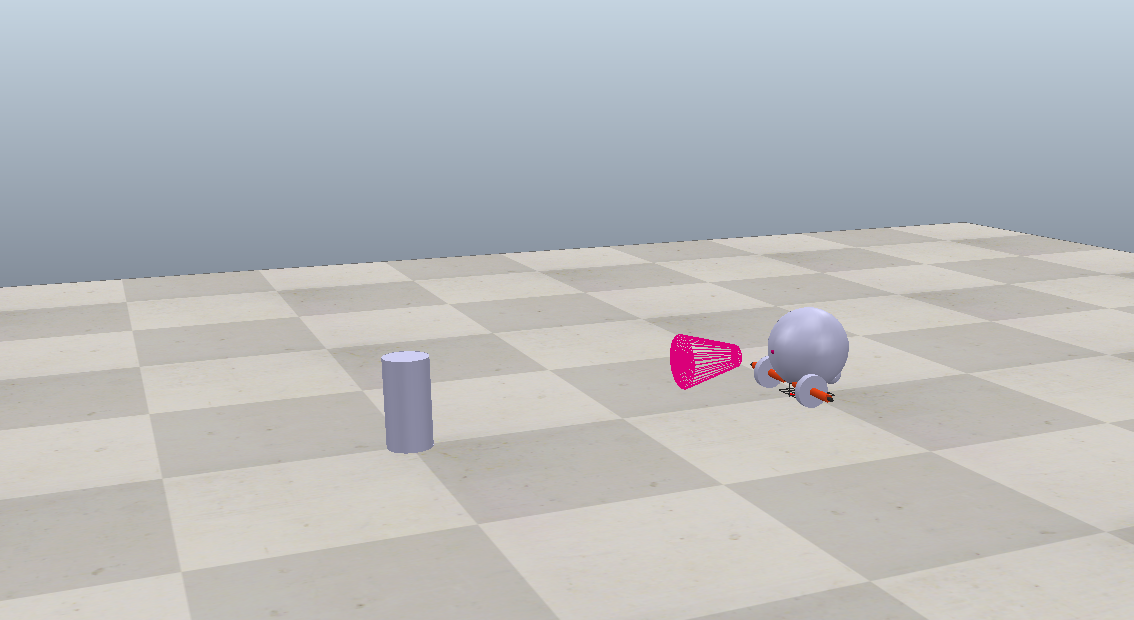
\includegraphics[width=16cm]{類神經網路架構}
\caption{\Large A}\label{A}
\end{center}
\end{figure}
\begin{center}
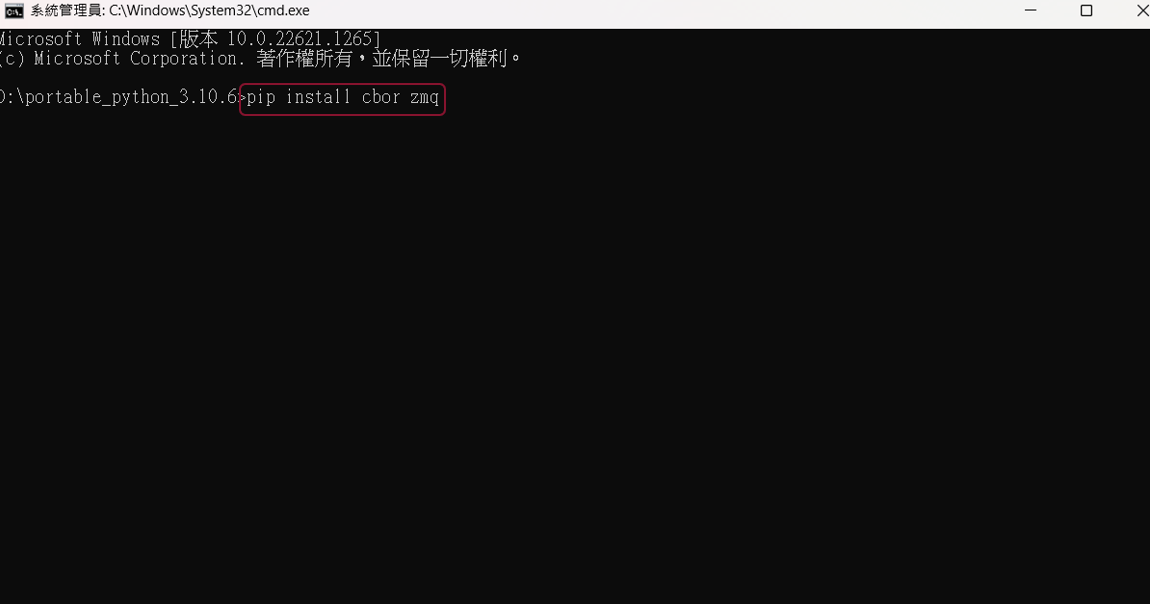
\includegraphics[width=16cm]{類神經網路關係}
\caption{\Large B}\label{B}
\end{center}
\end{figure}
 CoppeliaSim 自 4.3 版之後除了 Lua scripting, 增加了 Python scripting 功能. 但是必須在 usrset.txt 中設定 defaultPython 指向 Python.exe, pip install cbor zmq, 並且設定 executeUnsafe = true. 完成後開啟 CoppeliaSim 4.3.0 rev12, 並利用 scenes/simplePythonExample.ttt 進行測試如(圖.\ref{A})及(圖.\ref{B}) 。\\
\newpage
\begin{figure}
\begin{center}
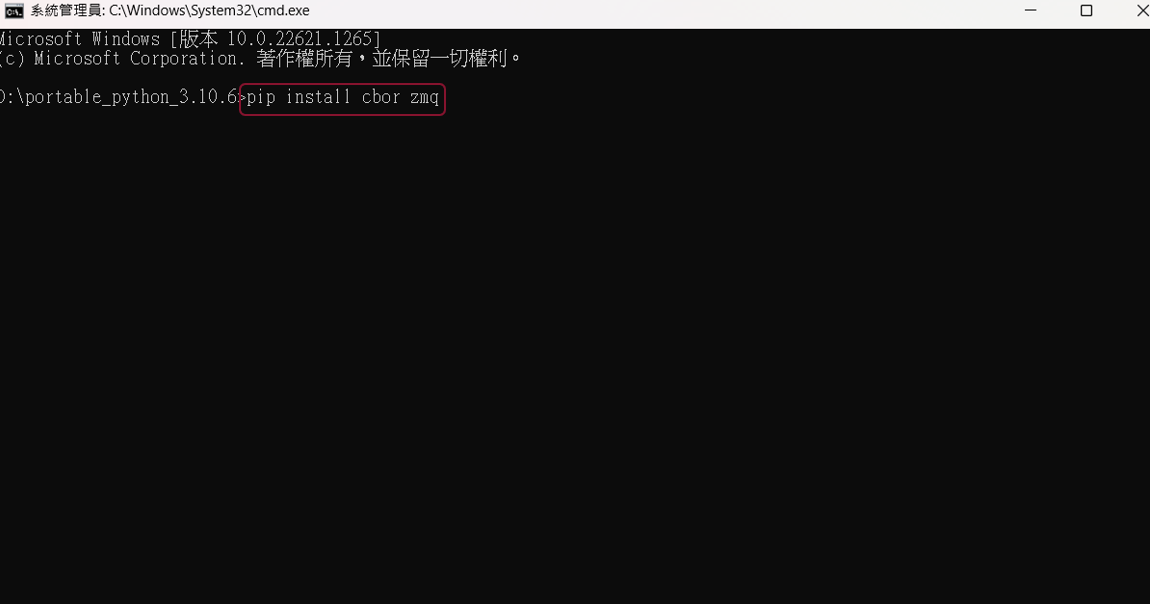
\includegraphics[width=16cm]{類神經網路關係}
\caption{\Large 類神經網路關係}
\label{類神經網路關係}
\end{center}
\end{figure}
\subsection{啟動函數}
啟動函數是設計類神經網路的關鍵部分,如果不使用啟動函數,神經元的計算只會有線性組合,這樣的類神經網路缺乏活性而且記憶性差;啟動函數能讓神經元計算呈現非線性,讓類神經網路因為計算的非線性而提高整個網路的活性和記憶性。\\
以下介紹幾種較為常見的啟動函數及其特性:
\begin{itemize}
%=----------Sigmoid      Function----------=%
\item Sigmoid Function(圖.\ref{SigmoidFunction}):\\
輸出介於0到1之間,適用於二元分類,方程式具有非線性、可連續微分、且具有固定輸出範圍等特性,並可以讓類神經網路呈現非線性。
$$\sigma(x)=\frac{1}{1+e^{-x}}$$

%=----------SigmoidPrime Function----------=%
SigmoidPrime Function(圖.\ref{SigmoidFunction},紅色的)是從Sigmoid Function(圖.\ref{SigmoidFunction},藍色)微分得來,以梯度運算的方式,可以減少梯度誤差,但也是造成梯度消失的主要原因,若要改善梯度消失需要搭配優化器使用,方程式如下:\\
$$\sigma^{'}(x)=\sigma(x)[1-\sigma(x)]$$
\begin{figure}[hbt!]
\begin{center}
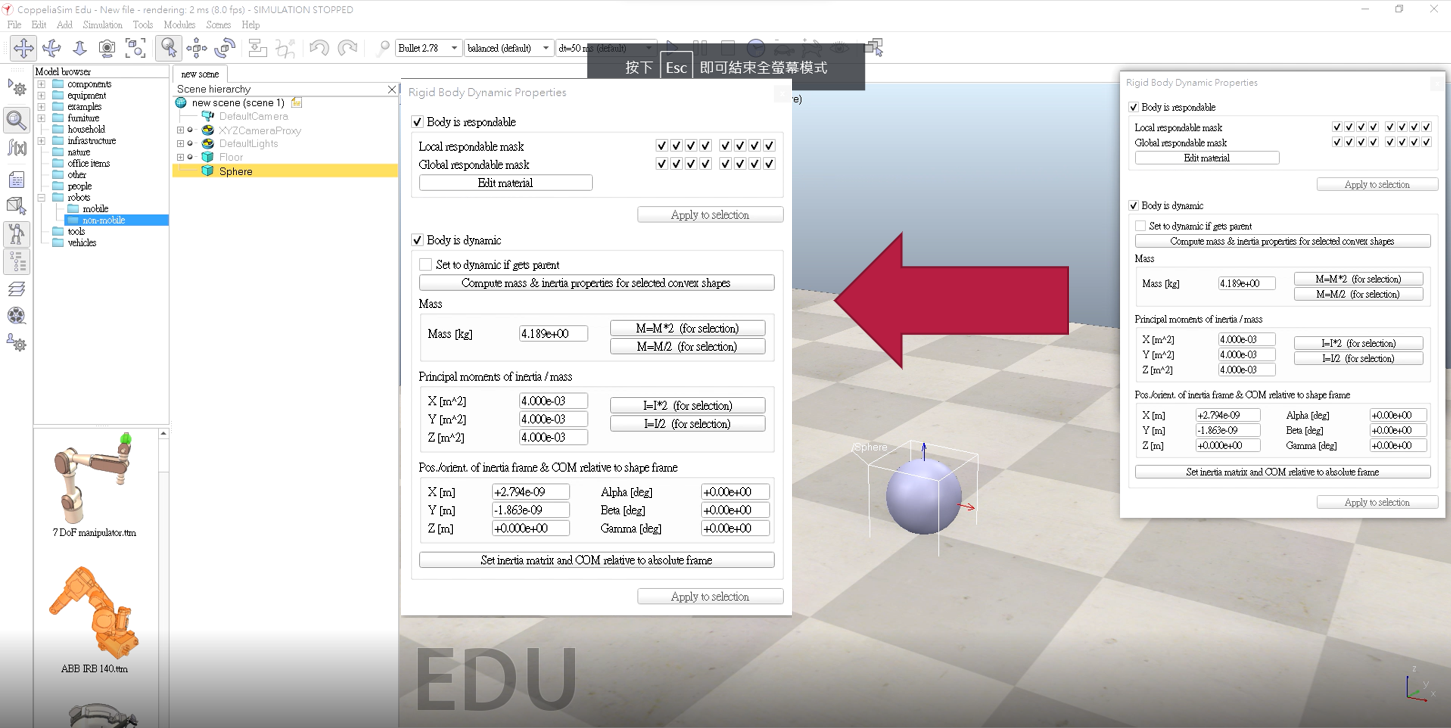
\includegraphics[width=16cm]{SigmoidFunction}
\caption{\Large SigmoidFunction}\label{SigmoidFunction}
\end{center}
\end{figure}
\\
%=----------Softmax Function----------=%
\item Softmax:\\
Softmax會計算每個事件分布的機率,適用多項目分類、其機率總合為1。以此專案為例,假設擊錘移動有向上移動、向下移動及不移動這三個決策選項,則這三個決策機率值總和為1。\\
$$S(x)=\frac{e^{x_i}}{\sum^k_{j=1}e^{x_i}}$$
%=----------Relu Function----------=%
\item ReLU Function:\\
ReLU Function方程式特性:若輸入值為負值,輸出值為0;若輸入值為正值,輸出則維持該輸入數值。ReLU計算方式簡單、收斂速度快,這是類神經網路最普遍拿來使用的啟動函數,因為可以解決梯度消散的問題,但須注意:起始值若設定到不易被激活範圍或是權重過渡所導致權重梯度為0就會造成神經元難以被激活。\\
\end{itemize}
$$f(x)=max(0,x)$$
$$if , x<0 , f(x)=0$$
$$else f(x)=x$$
\subsection{損失函數}
損失函數是類神經網路的另一個重要的部分,損失函數會將類神經網絡的結果與期望結果進行比較,且必須重複估算模型當前狀態的誤差;該函數可用於估計模型的損失,以便可以更新權重減少下次評估時的損失,下一節會有詳細說明,以下簡述幾種優化的方法:\\
\begin{itemize}
\item Gradient Descent\\
利用梯度的方式尋找最小值的位置,其特色可找到凸面error surface的絕對最小值,在非凸面error surface上找到相對最小值。其缺點是在非凸面error surface要避免被困在次優的局部最小值。
\item Batch gradient descent\\
用批次的方式計算訓練資料,整個資料集計算梯度只更新一次,因此計算和更新時會占用大量記憶體。整體效率較差、速度較緩慢。由 Gradient Descent 延伸出來的算法。其收斂行為與 Gradient Descent 相同。
\item Stochastic gradient descent\\
每次執行時會更新並消除誤差,有頻繁更新和變化大的特性,較不容易困在特定區域。由 Gradient Descent 延伸出來的算法。其收斂行為與 Gradient Descent 相同。
\item Mini-batch gradient descent\\
結合 Batch gradient descent 和 Stochastic gradient descent 的特點:批量計算和頻繁更新,所衍伸的算法。利用小批量的方式頻繁更新,並使收斂更穩定。其缺點:學習率挑選不易、預定義 threshold 無法適應數據集的特徵、對很少發生的特徵無法執行較大的更新、非凸面error surface要避免被困在次優的局部最小值等。
\item Gradient descent optimization algorithms\\
為了改善前面幾種算法而發展出來的優化算法。以下將列出數種優化算法。
\item Momentum\\
在梯度下降法加上動量的概念,會加速收斂到最小值並減少震盪。
\item Nesterov accelerated gradient\\
NAG,有感知能力的 Momentum:在坡度變陡時減速,避免衝過最小值所造成的震盪(為了修正到最小值,來回修正而產生的震盪)。
\item Adagrad\\
其學習率能適應參數:頻繁出現的特徵用較低的學習率,不經常出現的特徵則用較高的學習率,且無須手動調整學習率。其缺點是,學習率會急遽下降,最後會無限小,這算法就不再獲得知識。
\item Adadelta\\
為 Adagrad 的延伸,下降激進程度,學習率從更新規則中淘汰,不需設定預設學習率。
\item RMSprop\\
為了解決 Adagrad 學習率急劇下降的問題,學習率除以梯度平方的RMS,解決學習率無限小的情形。
\item Adam Function\\
結合了 Adagrad 和 RMSprop的優勢,有論文表示,在訓練速度方面有巨大性的提升,但在某些情況下,Adam實際上會找到比隨機梯度下降法更差的解決方法。以下是計算過程:\\
$$g_t=\delta_{\theta}f(\theta)$$
一次矩指數移動均線 :\\
$$m_t =\beta(m_{t-1})+(1-\beta_1)(\nabla{w_t})$$
$$\hat m_t=\frac{m_t}{1-\beta_1^t}$$
二次矩指數移動均線 :\\
$$v_t=\beta_2(v_t-1)+(1-\beta_2)(\nabla{w_t})^2$$
$$\hat{v_t}=\frac{v_t}{1-\beta_2^t}$$
因此,Adam Function:\\
$$\omega_{t-1}=\omega_t-\frac{\eta}{\sqrt{\hat{v_t}-\epsilon}}\hat{m_t}$$
\item AdaMax\\
與 Adam 相似,依靠$(u_t)$ 最大運算。
\item Nadam\\
結合 Adam 和 NAG ,應用先前參數執行兩次更新,一次更新參數一次更新梯度。
\item AMSGrad\\
改善 Adam 算法所導致收斂較差的情況(用指數平均會減少其影響),換用梯度平方最大值來做計算,並移除去偏差的步驟。是否有比 Adam 算法好仍有待觀察。
\item Gradient noise\\[6pt]
有助於訓練特別深且復雜的網絡,noise 可改善不良初始化的網路。
\item Mean Squared Error\\
他能告訴你一組點與回歸線接近的程度,透過獲取點與回歸線之距離(這些距離就是誤差)並對它們進行平方來做到這點,而平方是為了消除所有負號,也能讓更大的差異賦予更大的權重。\\
\vspace{8cm}
\begin{figure}
\begin{center}
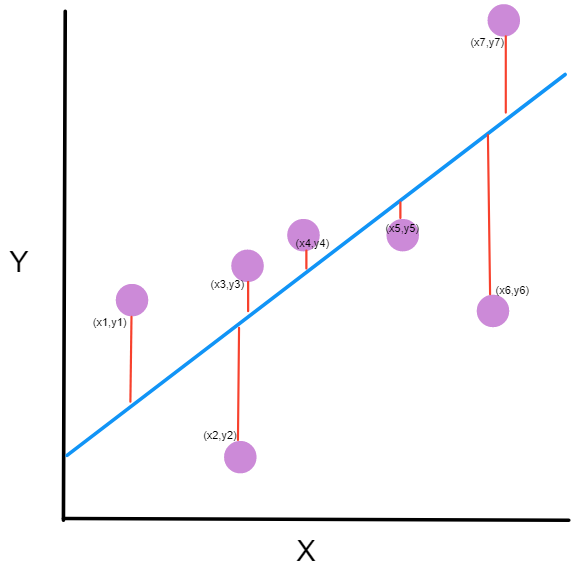
\includegraphics[scale=0.6]{MSE}
\caption{\Large 線性回歸}\label{線性回歸}
\end{center}
\end{figure}
\qquad \\

回歸線 :數據點間最小距離的一條線。 \\
n:數據點的數量\\
$y_i$: 觀測值\\
$\hat{y_i}$:預測值\\
$$MSE=\frac{1}{n} \sum_{i=1}^n(y_i-\overline{y} _i)^2$$\\
\end{itemize}
\newpage
\subsection{優化算法}
\renewcommand{\baselinestretch}{1}

\begin{itemize}
\item Gradient Descent Optimizer[\ref{OGD}]\\

\begin{figure}[hbt!]
\begin{center}
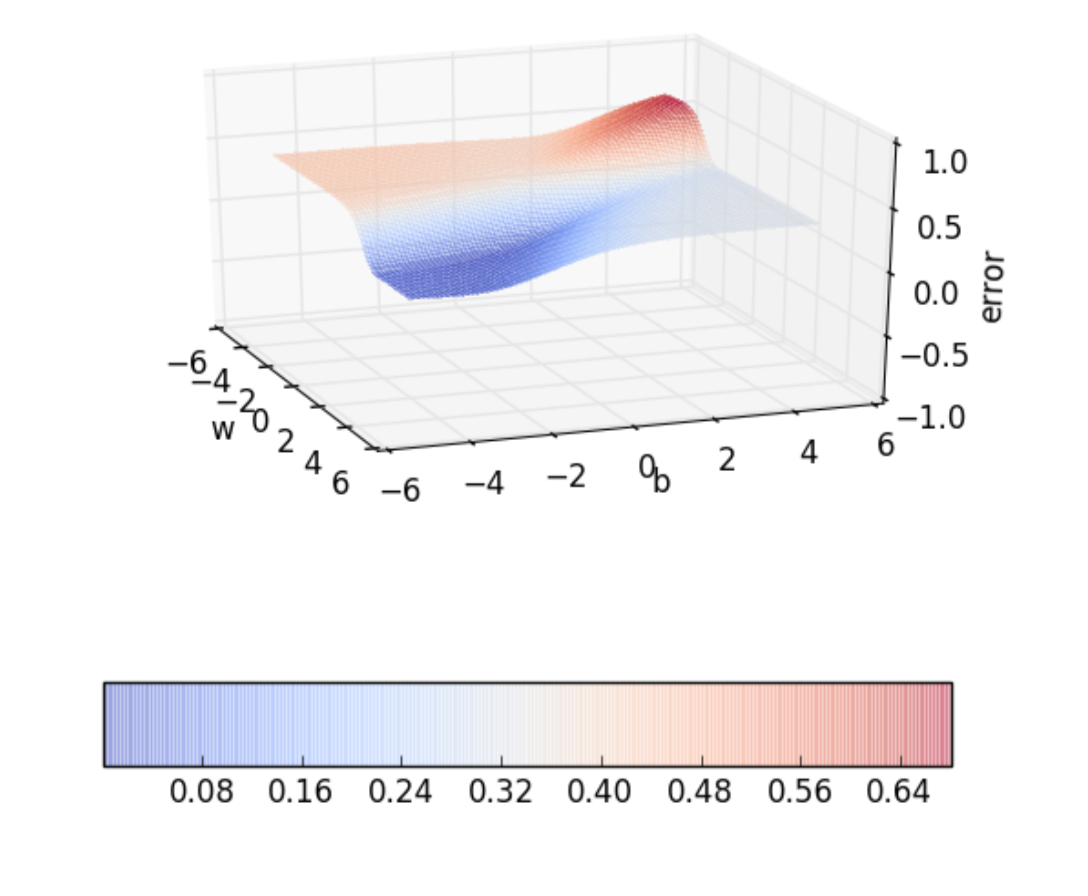
\includegraphics[width=10cm]{Error_surface-2}
\caption{\Large Error surface [\ref{OGD}]}
\label{Error_surface-2}
\end{center}
\end{figure}
%\fontsize{14pt}{28pt}\selectfont
 藉由梯度下降將目標函數值最小化,目標函數以loss function L($\theta$)為例,$\theta$為weight(w)和bias(b)的向量函數,為了找到(圖.\ref{Error_surface-2})上的最小值,因此加上$\Delta\theta$將$\theta$ 的方向修正並引導到正確方向,避免每次修正的過多導致錯過最小值,利用係數$\eta$(學習率)縮放$\Delta\theta$的修正量(圖.\ref{theta_vector}),修正後方程式為:
$$\theta=\theta+\eta\cdot\Delta\theta$$
\begin{figure}
\begin{center}
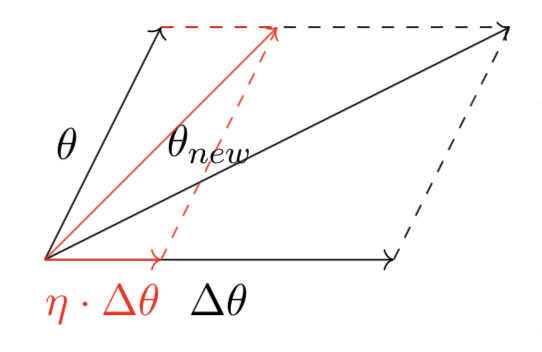
\includegraphics[width=10cm]{theta_vector}
\caption{\Large theta vector[\ref{OGD}]}
\label{theta_vector}
\end{center}
\end{figure}
\newpage
將$\theta$以泰勒展開式表示,假設並$\Delta\theta$為u:
\begin{center}
$L_{(\theta+\eta u)}=L_{(\theta)}+\eta u^{T}\cdot\bigtriangledown_{\theta} L_{(\theta)}+\frac{\eta^2}{2!}u^T\cdot\bigtriangledown^2 L_{(\theta)}u+\frac{\eta^3}{3!}...+\frac{\eta^4}{4!}...+\frac{\eta^n}{n!}...$\\
\end{center}
以泰勒展開式的型式表示的好處是:$\theta$些微的更動產生新值。$\eta$值通常小於一,當$\eta^2 << 1$,因此可以忽略高階項 
\begin{center}
$L_{(\theta+\eta u)}=L_{(\theta)}+\eta u^{T}\cdot\bigtriangledown_{\theta} L_{(\theta)} [\eta\ is\ typically\ small, so\ \eta^2, \eta^3,\cdots \rightarrow 0]$\\
\end{center}
新的$L(\theta + \eta u)$輸出的值會小於$L(\theta) L(\theta+\eta u) − L(\theta) < 0$,同理可證$u^T\cdot\bigtriangledown\theta L(\theta)$,符合u這條件:當新的值小於舊的值,u就是一個好的值。假設u和$\bigtriangledown\theta L(\theta)$的夾角為$\beta$\\
\begin{center}
$\cos(\beta)=\frac{u^{T}\cdot\bigtriangledown_{\theta} L_{(\theta)}}{\vert u^{T}\vert\vert \bigtriangledown_{\theta} L_{(\theta)}\vert}$\\
\end{center}
因為$\cos(\theta)$的值介於1和-1之間\\
\begin{center}
$-1<\cos(\beta)=\frac{u^{T}\cdot\bigtriangledown_{\theta} L_{(\theta)}}{\vert u^{T}\vert\vert \bigtriangledown_{\theta} L_{(\theta)}\vert}\leq 1$\\
$k=\vert u^{T}\vert\vert \bigtriangledown_{\theta} L_{(\theta)}\vert$\\
$-k \leq k\cos(\beta)=u^{T}\cdot\bigtriangledown_{\theta} L_{(\theta)}\leq k$
\end{center}
\newpage
 所以盡可能的讓新值小於舊值$(L(\theta+\eta u) − L(\theta) < 0)$,loss 值就會減少得越多。因此$u T \cdot \bigtriangledown\theta L(\theta)$應該為負,在這情況下$\cos(\beta)$於−1,$\beta$的角度為 $180^{\circ}$這就是$\theta$移動的方向與梯度方向相反的原因。 梯度下降法告訴我們:當$\theta$在特定值,並想減少新的$\theta$值,使 loss 值逐漸減少就應該與梯度相反的方向找 (若梯度為正值,找最小值就需往負的方向找):
\begin{center}
$w_{t=1}=w_t-\eta\bigtriangledown w_t$\\
$b_{t=1}=b_t-\eta\bigtriangledown b_t$\\
$where\ at\ w=w_t,b=b_t$\\
$\begin{cases}
 \bigtriangledown w_t=\frac{\partial L_{_{(\theta)}}}{\partial w}
 \bigtriangledown b_t=\frac{\partial L_{_{(\theta)}}}{\partial b}
 \end{cases}$
\end{center}
\item Batch gradient descrnt [\ref{OGD2}]\\
 Vanilla gradient descent 又稱 Batch gradient descent(批次梯度下降法),計算目標函數的梯度,參數$\theta$對於整個 訓練資料:
\begin{center}
$\theta=\theta-\eta\cdot\bigtriangledown_{\theta}L_{(\theta)}$
\end{center}
 目標函數以為例 loss function L($\theta$),參數$\theta$為 weight(w)和 bias(b)的函數,$\eta$為學習率。由於計算整個資料集計算梯度只更新一次,Bath gradient descent 可能非常慢並且對於資料集無法符合及記憶體來說棘手(一次需要儲存整個資料集的資料,當更新和計算時會占用大量記憶體)。\\
\begin{lstlisting}[caption=\Large Batch gradient descrnt]
 for i in range(nb_epochs) :
params_grad = evaluate_gradient (loss_function, data, params)
params = params − learning_rate * params_grad
\end{lstlisting}
\newpage
 預定義每次epoch,先計算loss function梯度向量對於整個資料集參數向量。如果梯度值來自於先前計算出的梯度值,就會檢查梯度,並以梯度相反的方向更新參數$\theta$,學習率$\eta$決定多大的更新量。Batch gradient descent對於凸面誤差可以保證收斂到廣域最小值,對於非面凸誤差可以收斂到局部最小值。
\item Stochastic gradient descent(SGD)[\ref{OGD2}]\\
隨機梯度下降法,這裡的目標函數為$J(\theta, x^i, y^i)$(變數$\theta$為 w(weight) 和 b(bias) 的函數,也可以寫成$J(w,b,\theta, x^i, y^i)$)。\\
\begin{center}
$\theta=\theta-\eta\cdot\bigtriangledown_{\theta}J_{(\theta, x^i, y^i)}$
\end{center}
批量梯度下降他會在每個參數更新前重新計算相似梯度。SGD 每次次執行會更新來消除多餘 (誤差),因此通常速度 很快。SGD 頻繁更新並變化很大,因為目標方程式波動很大(圖.\ref{sgd_fluctuation})。\\

\begin{figure}
\begin{center}
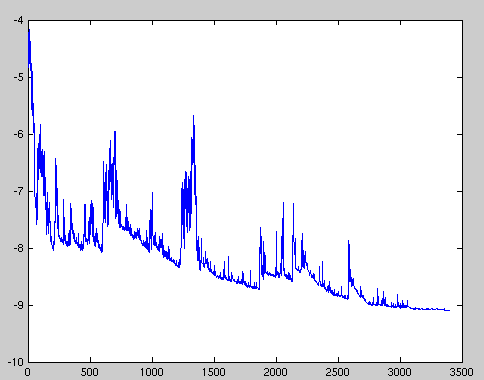
\includegraphics[width=10cm]{sgd_fluctuation}
\caption{\Large SGD fluctuation[\ref{OGD2}]}
\label{sgd_fluctuation}
\end{center}
\end{figure}
 SGD 的方程式一方面會跳到新的值和潛在局部最小值,另一方面 SGD 會持續超調 (誤差超過預期) 最後收斂到廣域最小值。無論如何他被顯示當學習率下降緩慢,SGD 顯示與 Batch gradient descent 同樣收斂行為,幾乎可以肯定地,對於凸面或非凸面優化,會收斂到絕對或是局部最小值。這程式碼片段[程式.2.2] 在訓練樣本上加入一個迴圈來對每個樣本評估梯度。每個 epoch(訓練循環) 會打亂訓練數據。
\label{code Stochastic gradient descrnt code}
\begin{lstlisting}[caption=\Large Stochastic gradient descrnt ]
for i in range(nb_epochs) :
np.random.shuffle(data)
for example in data :
params_grad = evaluate_gradient (loss_function, example, params)
params = params − learning_rate * params_grad
\end{lstlisting}
\item Mini-batch gradient descent[\ref{OGD2}]

 Mini-batch gradient descent(小批量梯度下降) 各取前兩者的優點,將資料集分割成小區塊,每個小區塊大小稱作 batch size,每次跑完 batch size 算迭代 (iteration)一次,算完一次資料集即完成一次 epoch。舉例: 資料集大小為1000,若 batch size 為50,iteration 為 datasets 的batch size  = 1000÷50 = 20,當 iteration 跑完 20 次算完成一次 epoch。\\
這方式可以減少參數更新的方差,並且可以穩定收斂;可利用深度學習庫所共有的高度優化的矩陣優化,從而由一個小批量計算出梯度非常有效。通常 batch sizes 的範圍介於 50 ~256,會因為應用而有所差異。訓練神經網絡時,通常選擇 Mini-batch gradient descent 算法,而當使用這算法時,通常也用 SGD 稱呼。\\
\begin{center}
$\theta=\theta-\eta\cdot\bigtriangledown_{\theta}J_{(\theta, x^{(i:i+n)}, y^{(i:i+n)})}$
\end{center}
下面[程式.2.3] 為迭代範例,batch size 大小為 50:\\
\label{Mini-batch gradient descrnt}
\begin{lstlisting}[caption=\Large Mini-batch gradient descrnt]
for i in range(nb_epochs ) :
np.random.shuffle(data)
for batch in get_batches (data, batch_size = 50):
params_grad = evaluate_gradient (loss_function, batch, params)
params = params − learning_rate ∗ params_grad
\end{lstlisting}
Mini-batch gradient descent 無論如何還是無法確保收斂的很好,存在一些需要解決的挑戰:
\begin{enumerate}[1]
\item 選擇適當的學習率是有難度的。如果學習率太小會導致收斂困難或緩慢,學習率太大則會阻礙收斂導致 loss function 來回波動或發生偏離。
\item 學習率清單嘗試在訓練的時候調整學習率,即根據預定義清單或當目標下降於閾值 (threshold) 時降低學習率。 但清單和閾值須預先定義,因此無法適應數據集的特徵。
\item 另外相同學習率適用全部參數更新。如果資料稀疏而且外型有很特別的頻率,我們可能不希望將所有特徵更新 到相同的程度,而是對很少發生的特徵執行較大的更新。
\item 最小化神經網路常見的高度非凸面誤差方程式 (error function) 的另一關鍵挑戰則是要避免被困在大量次優的局 部最小值區域中。認為困難實際上不是由局部最小值引起的,而是由鞍點引起的,即一維向上傾斜而另一維向下 傾斜的點。這些鞍點通常被相同誤差的平穩段包圍,這使得 SGD 很難逃脫,因為在所有維度上梯度都接近於零。
 \end{enumerate}
\item Gradient descent optimization algorithms[\ref{OGD2}]\\
SGD 難以在陡峭的往正確的方向,那就是說在一個維度上,曲面的彎曲比另一個維度要陡得多,這在局部最優情況下很常見。下圖(圖.1)的同心圓代表中心下凹的曲面。在這些情況下,SGD 會在陡峭的地方振盪,而僅沿著底部朝著局部最優方向猶豫前進,如(圖.\ref{fig.without_momentum}) 所 示。 Momentun(動量) 是一個幫助加速 SGD 在正確方向和抑制震盪的方法,在(圖.\ref{fig.with_momentum})。\\

\begin{figure}[hbt!]
\begin{center}
\subfigure{
\begin{minipage}[t]{0.5\linewidth}  %設定圖片間距
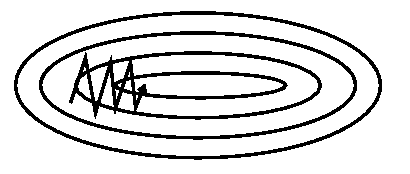
\includegraphics[width=6cm]{without}
\caption{\Large SGD without momentum[\ref{OGD2}]}
\label{fig.without_momentum}
\end{minipage}
}
\subfigure{
\begin{minipage}[t]{0.5\linewidth}
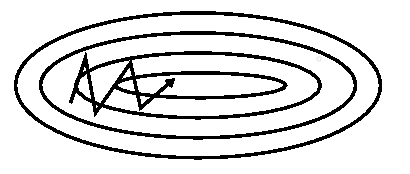
\includegraphics[width=6cm]{with}
\caption{\Large SGD with momentum[\ref{OGD2}]}
\label{fig.with_momentum}
\end{minipage}
}
\end{center}
\end{figure}

這麼做會增加一個係數$\gamma$來更新上次的向量到正確向量 (修正偏差),$\gamma$通常設為 0.9 左右。
\begin{center}
$v_t = \gamma v_{t-1}+\eta\cdot\bigtriangledown_{\theta}J_{(\theta)}$
$\theta = \theta-v_t$
\end{center}
 實際上,使用動量的時候,就像將球推下山坡。球在下坡時滾動時會累積動量,在途中速度會越來越快(如果存在空氣阻力,直到達到極限速度,也就是$\gamma < 1$) 參數更新也發生了同樣的事情:動量 (momentum) 對於梯度指向相同方向的維度增加,而對於梯度改變方向的維減少動量。結果,我們獲得了更快的收斂並減少了振盪。\\

 Nesterov accelerated gradient(NAG)是一種使動量具有一個去向的概念,以便在山坡再次變高之前知道它會減速。我們知道使用動量$\gamma v_{t-1}$來移動參數。計算$\theta - \gamma v_{t-1}$這樣就給了參數的下一個位置的近似值(完整更新缺少的梯度),這是參數將要存在的大致概念。現在,通過計算與當前參數無關的梯度來有效地看到目前的參數$theta$將會移動到的位置:
\begin{center}
$v_t = \gamma v_{t-1}+\eta\cdot\bigtriangledown_{\theta}J_{(\theta-\gamma v_{t-1})}$
$\theta = \theta - v_t$
\end{center}

\begin{figure}[hbt!]
\begin{center}
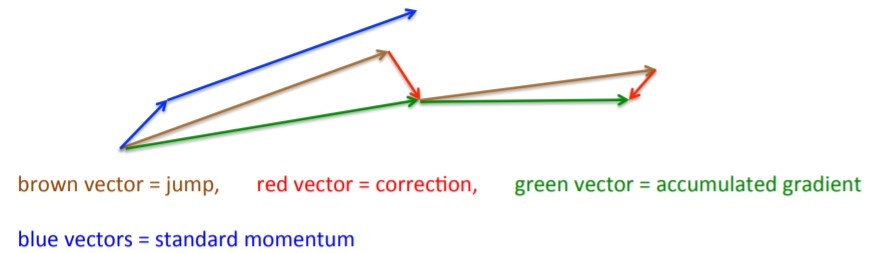
\includegraphics[width=13cm]{NAG}
\caption{\Large NAG[\ref{OGD2}]}
\label{NAG}
\end{center}
\end{figure}
同樣,我們設置動量$\gamma$約為0.9。動量首先計算當前梯度((圖.\ref{NAG})中的藍色小向量),然後在更新的累積梯度(藍 色向量)的方向上發生較大的跳躍,而 NAG 首先在先前的累積梯度的方向上進行較大的跳躍(棕色向量),測量梯度,然後進行校正(紅色向量),從而完成 NAG 更新(綠色向量)。這種預期的更新可防止我們過快地進行,並導致響應速度增加,從而顯著提高了 RNN 在許多任務上的性能。\\
Adagrad[\ref{OGD2}]:\\
 Adagrad 是一個梯度優化的算法,它可以做到:學習率適應參數,對於頻繁出現的特徵相關參數執行較小的更新(較低的學習率),以及對不經常出現的特徵相關參數進行較大更新(即學習率較高)。Adagrad可以提高SGD的強度,用於訓練大型神經網絡。\\
 先前,在同一次$theta$參數(更新後就算另一次),每個$theta$都使用相同的$\eta$(學習率)。Adagrad 則是對每個$theta$參數使用 不同的$\eta$,t 代表 time step。先將 Adagrad 的更新參數向量化。用$g_t$表示目標函數 (參數$theta$在 time step t) 對參數做偏微分計算。
\begin{center}
$g_{t,i}=\bigtriangledown_{\theta}J_{(\theta_{t,i})}$
\end{center}
當 SGD 更新每個參數$\theta_i$,在每個 time step t,因此變成:
\begin{center}
$\theta_{t+1,i}=\theta_{t,i}-\eta\cdot g_{t,i}$
\end{center}
更新規則,Adagrad 根據先前$\theta_i$計算的梯度,對每個參數$\theta_i$修改整個學習率$\eta$在每個 time stept:
\begin{center}
$\theta_{t+1,i}=\theta_{t,i}-\frac{\eta}{\sqrt{G_{t,ii}+\epsilon}}$
\end{center}
$G_t \in \mathbb{R}^{d\times d}$這是一個對角矩陣每個對角元素 i,i 是關於$theta$梯度平方和取決於 time stept,$\epsilon$是避免分母為0($\epsilon$通常為$10^{-8}$),如果沒有平方根運算,該算法的性能將大大降低。$G_t$包含了過去梯度平方根,由於全部$theta$參數沿著對角線,通過向量的內積計算$G_t$和$g_t$:
\begin{center}
$\theta_{t+1}=\theta_{t}-\frac{\eta}{\sqrt{G_{t}+\epsilon}}\cdot g_t$
\end{center}
 Adagrad 主要好處之一是,無需手動調整學習率。大多數實現使用預設值 0.01 並將其保留為預設值。Adagrad主要弱點是會累積分母的平方梯度:由於每項都是正的,累積和會在訓練中不斷增長。反過來,學習率下降,並最終變得無限小,這算法就不再獲得知識。\\
Adadelta[\ref{OGD2}]:\\
 Adadelta是Adagrad的延伸,下降其激進的程度,單調的降低學習率。Adadelta會限制過去累積的梯度,並將其限制在某個特定大小 w,並代替Adagrad過去累積的梯度平方,以梯度總和是遞迴定義為所有過去衰減梯度平方平均值。流動平均$E[g^2]_t$ 在time stept然後取決於(像Momentum的$\gamma$)先前平均和最近梯度:
\begin{center}
$E[g^2]_t=\gamma E[g^2]_{t-1}+(1-\gamma)g^2 _t$
\end{center}
$\gamma$值和 Momentum 的相似,約為 0.9,現在根據參數更新向量$\bigtriangleup\theta_t$來重寫 SGD:
\begin{center}
$\bigtriangleup\theta_t=-\eta\cdot g_{t,i}$\\
$\theta_{t+1}=\theta_t+\bigtriangleup\theta_t$
\end{center}
Adagrad 的參數更新向量替換成:對角矩陣$G_t$過去梯度平方的衰退平均$E[g^2]_t$
\begin{center}
$\bigtriangleup\theta_t=-\frac{\eta}{\sqrt{G_t+\epsilon}}\cdot g_t$\\
$replace\ G_t\ with\ E[g^2]_t\Rightarrow\bigtriangleup\theta_t=-\frac{\eta}{\sqrt{E[g^2]_t+\epsilon}}\cdot g_t$
\end{center}
由於分母只是梯度的均方根 (RMS),我們可以取代成縮寫:
\begin{center}
$\bigtriangleup\theta_t=-\frac{\eta}{RMS[g]_t}\cdot g_t$
\end{center}
 這個更新單位和 SGD、Momentum 以及 Adagrad 的單位不符合,因此更新需有相同的參數。為了實現這一點,首先定義另一個指數衰減平均值,這次不是梯度平方更新而是參數平方更新:
\begin{center}
$E[\bigtriangleup\theta^2]_t=\gamma E[\bigtriangleup\theta^2]_{t-1}+(1-\gamma)\bigtriangleup\theta^2 _t$
\end{center}
RMS 參數更新:
\begin{center}
$RMS[\bigtriangleup\theta]_t=\sqrt{E[\bigtriangleup\theta^2]_t+\epsilon}$
\end{center}
$RMS[\bigtriangleup\theta]_t$是未知的,更新參數的 RMS 取近似值到上個 time step。用$RMS[\bigtriangleup\theta]_t$取代學習率$\eta$,最後產生新的規則:
\begin{center}
$\bigtriangleup\theta_t=-\frac{RMS[\bigtriangleup\theta]_{t-1}}{RMS[g]_t}g_t$
\\
$\theta_{t+1}=\theta_t+\bigtriangleup\theta_t$
\end{center}
使用 Adadelta,甚至不需要設定預設學習率,因為它已從更新規則淘汰。\\
RMSprop[\ref{OGD2}]:\\
 RMSprop 是 Geoffrey Hinton 在他的課程中提出的未公開自適應學習率的方法。\\

 RMSprop 和 Adadelta 都是為了解決 Adagrad 的學習率急劇下降的問題個別獨立開發出來的解決方式。RMSprop 實際上與 Adadelta 得出的第一個更新向量相同:
\begin{center}
$E[g^2]_t=0.9E[g^2]_t+0.1g^2 _t$
\\
$\theta_{t+1}=\theta_t-\frac{\eta}{\sqrt{E[g^2]_t+\epsilon}}g_t$
\end{center}

 RMSprop 也將學習率除以梯度平方的指數衰減平均值。Hinton 建議$\gamma$設為 0.9,好的預設學習率$\gamma$數值為 0.001。\\
Adaptive Moment Estimation:[\ref{OGD2}]\\
 Adaptive Moment Estimation 自適應矩評估 (Adam) 是另一種計算每個評估學習率的方法。出了儲存過去梯度平 方的指數衰減平均值$v_t$,就像 Adadelta 和 RMSprop 一樣,Adam 還保留過去梯度的指數衰減平均值$m_t$,類似動量 (Momentum)。如果 Momentum 被視為順著斜坡下滑的球,而 Adam 則是像一個帶有摩擦的沉重的球,因此更適合待在 error face 平坦的最小值區域。計算過去梯度平方的衰減平均值$m_t$和$v_t$分別如下:
\begin{center}
$m_t=\beta_1 m_{t-1}+(1-\beta_1)g_t$\\
$v_t=\beta_2 v_{t-1}+(1-\beta_2)g^2 _t$
\end{center}
$m_t$和$v_t$分別是第一階矩平均估計值和第二階矩無中心方差估計值,因此是方法的名稱。像$m_t$和$v_t$被初始化為向量 o,Adam 的作者觀察到它們偏向零,特別是在初始 time step,尤其是在衰減率較小的時候 (也就是說$\beta_1$和$\beta_2$趨近於 1) 藉由計算校正偏差第一矩$\hat{m}_t$和第二矩$\hat{v}_t$抵消偏差:
\begin{center}
$\hat{m}_t = \dfrac{m_t}{1 - \beta^t_1}$\\
$\hat{v}_t = \dfrac{v_t}{1 - \beta^t_2}$
\end{center}
使用他們去更新參數,就像 Adadelta 和 RMSprop 中所看到的那樣,這將產生 Adam 更新規則:
\begin{center}
$\theta_{t+1} = \theta_{t} - \dfrac{\eta}{\sqrt{\hat{v}_t} + \epsilon} \hat{m}_t$
\end{center}
$\beta_1$預設值建議為 0.9,$\beta_2$預設值建議為 0.999,ϵ 預設值建議為$10^{-8}$。根據經驗證明 Adam 表現良好,並且與其他自適應學習算法相比具有優勢。
在 Adam 更新規則中的$v_t$係數是與梯度成反比地縮放過去梯度的範數 (通過 $v_{t-1}$項) 和當前梯度$|g_t|^2$:
\begin{center}
$v_t = \beta_2 v_{t-1} + (1 - \beta_2) |g_t|^2$
\end{center}
我們轉換這個更新到$\ell_p$。注意$\beta_2$參數化為$\beta_2^p$:
\begin{center}
$v_t = \beta_2^p v_{t-1} + (1 - \beta_2^p) |g_t|^p$
\end{center}
大規範 p 值使數值上變得不穩定,這就是為什麼$\ell_1$和$\ell_2$規範在實踐中是最常見的。然而$\ell_\infty$通常也表現出穩定 的行為。為了避免與 Adam 混用,所以使用$u_t$來表示無窮範數約束$v_t$:
\begin{center}
$u_t = \beta_2^\infty v_{t-1} + (1 - \beta_2^\infty) |g_t|^\infty$\\
$= \max(\beta_2 \cdot v_{t-1}, |g_t|)$
\end{center}
替換為Adam更新公式$\sqrt{\hat{v}_t} + \epsilon$和$u_t$得出AdaMax更新規則:
\begin{center}
$\theta_{t+1} = \theta_{t} - \dfrac{\eta}{u_t} \hat{m}_t$
\end{center}
替換為Adam更新公式$\sqrt{\hat{v}_t} + \epsilon$和$u_t$得出AdaMax更新規則:
\begin{center}
$\theta_{t+1} = \theta_{t} - \dfrac{\eta}{u_t} \hat{m}_t$
\end{center}
注意$u_t$依靠最大運算,不建議 Adam 中的$m_t$和$v_t$偏向零,這就是為什麼不需要針對$u_t$計算偏差。好的預設值$\eta = 0.002$ $\beta_1 = 0.9$ 和 $\beta_2 = 0.999$。\\
\end{itemize}


\section{強化學習}
%=----------What is Reinforcement Learning?------------=%
強化學習(Reinforcement Learning,簡稱為RL)是通過agent(代理)與已知或未知的環境持續互動,不斷適應與學習,會得到正向或負面的回饋,對應到獎賞(reward)和懲罰(punishments)。考慮到agent與環境(environment)互動,進而決定要執行哪個動作,強化學習的學習模式是建立在獎賞與懲罰上。\\

強化學習與其他學習法不一樣的地方在於:不需要事先收集大量數據提供當作學習樣本,而是透過與環境互動,在環境下發生的狀態當作學習的資料來源,透過不斷嘗試使所得到的獎勵最大化。其他類型的機器學習大都需要給予特定資料且有明確的答案。\\

由於強化學習是建立在agent與環境互動上,因此許多參數進行運算,需要大量資訊來學習,並根據資訊採取行動。強化學習的環境可以是真實世界、2D或3D模擬世界的場景。強化學習的範圍很廣,因為環境的規模可能很大,且在環境中有多相關因素,影響著彼此。強化學習以獎勵的方式,促使學習結果趨近或達到目標結果。\\
%=----------Faces of Reinforcement Learning---------------=%

強化學習涵蓋範圍(圖.\ref{各領域與機器學習應用範圍}):\\
 強化學習可以運用在計算機科學、神經科學、心理學、經濟學、數學、工程等領域,涵蓋領域相當廣泛。
%======需文字補充========%
\begin{figure}[hbt!]
\begin{center}
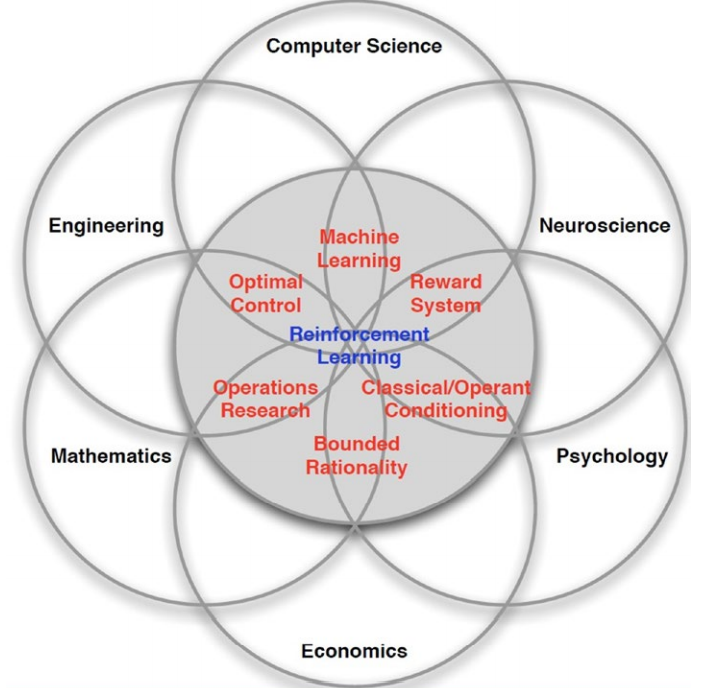
\includegraphics[width=11cm]{Faces_of_Reinforcement_Learning}
\caption{\Large 各領域與機器學習應用範圍}
\label{各領域與機器學習應用範圍}
\end{center}
\end{figure}
%=--------The Flow of Reinforcement Learning------------=%.
\newpage
強化學習的流程:\\
透過agent與環境間互動而產生狀態和獎勵,由於狀態的轉移,agent會決定接下來執行動作(圖.\ref{RL structur})。\\[12pt]

\begin{figure}[hbt!]
\begin{center}
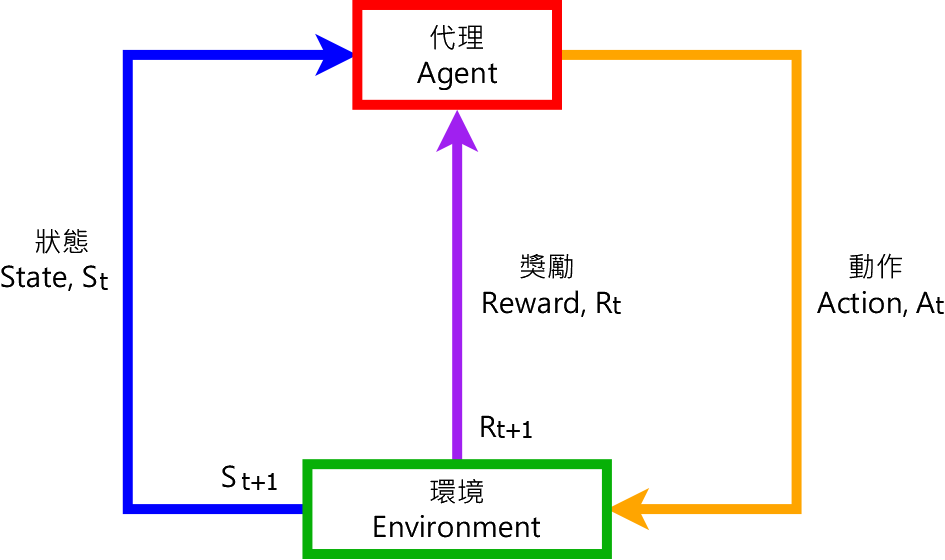
\includegraphics[width=12cm]{The_Flow_of_Reinforcement_Learning}
\caption{\Large 強化學習架構}
\label{RL structur}
\end{center}
\end{figure}
需要考慮的重點:\\
強化學習的狀態、獎勵和動作是互相關聯,agent與環境之間存在著關聯,兩者都影響著狀態和動作並互相影響著彼此:機器人會因動作而造成狀態轉移,狀態的移轉也會影響機器人做出的決策。\\
\newpage
\begin{figure}[hbt!]
\begin{center}
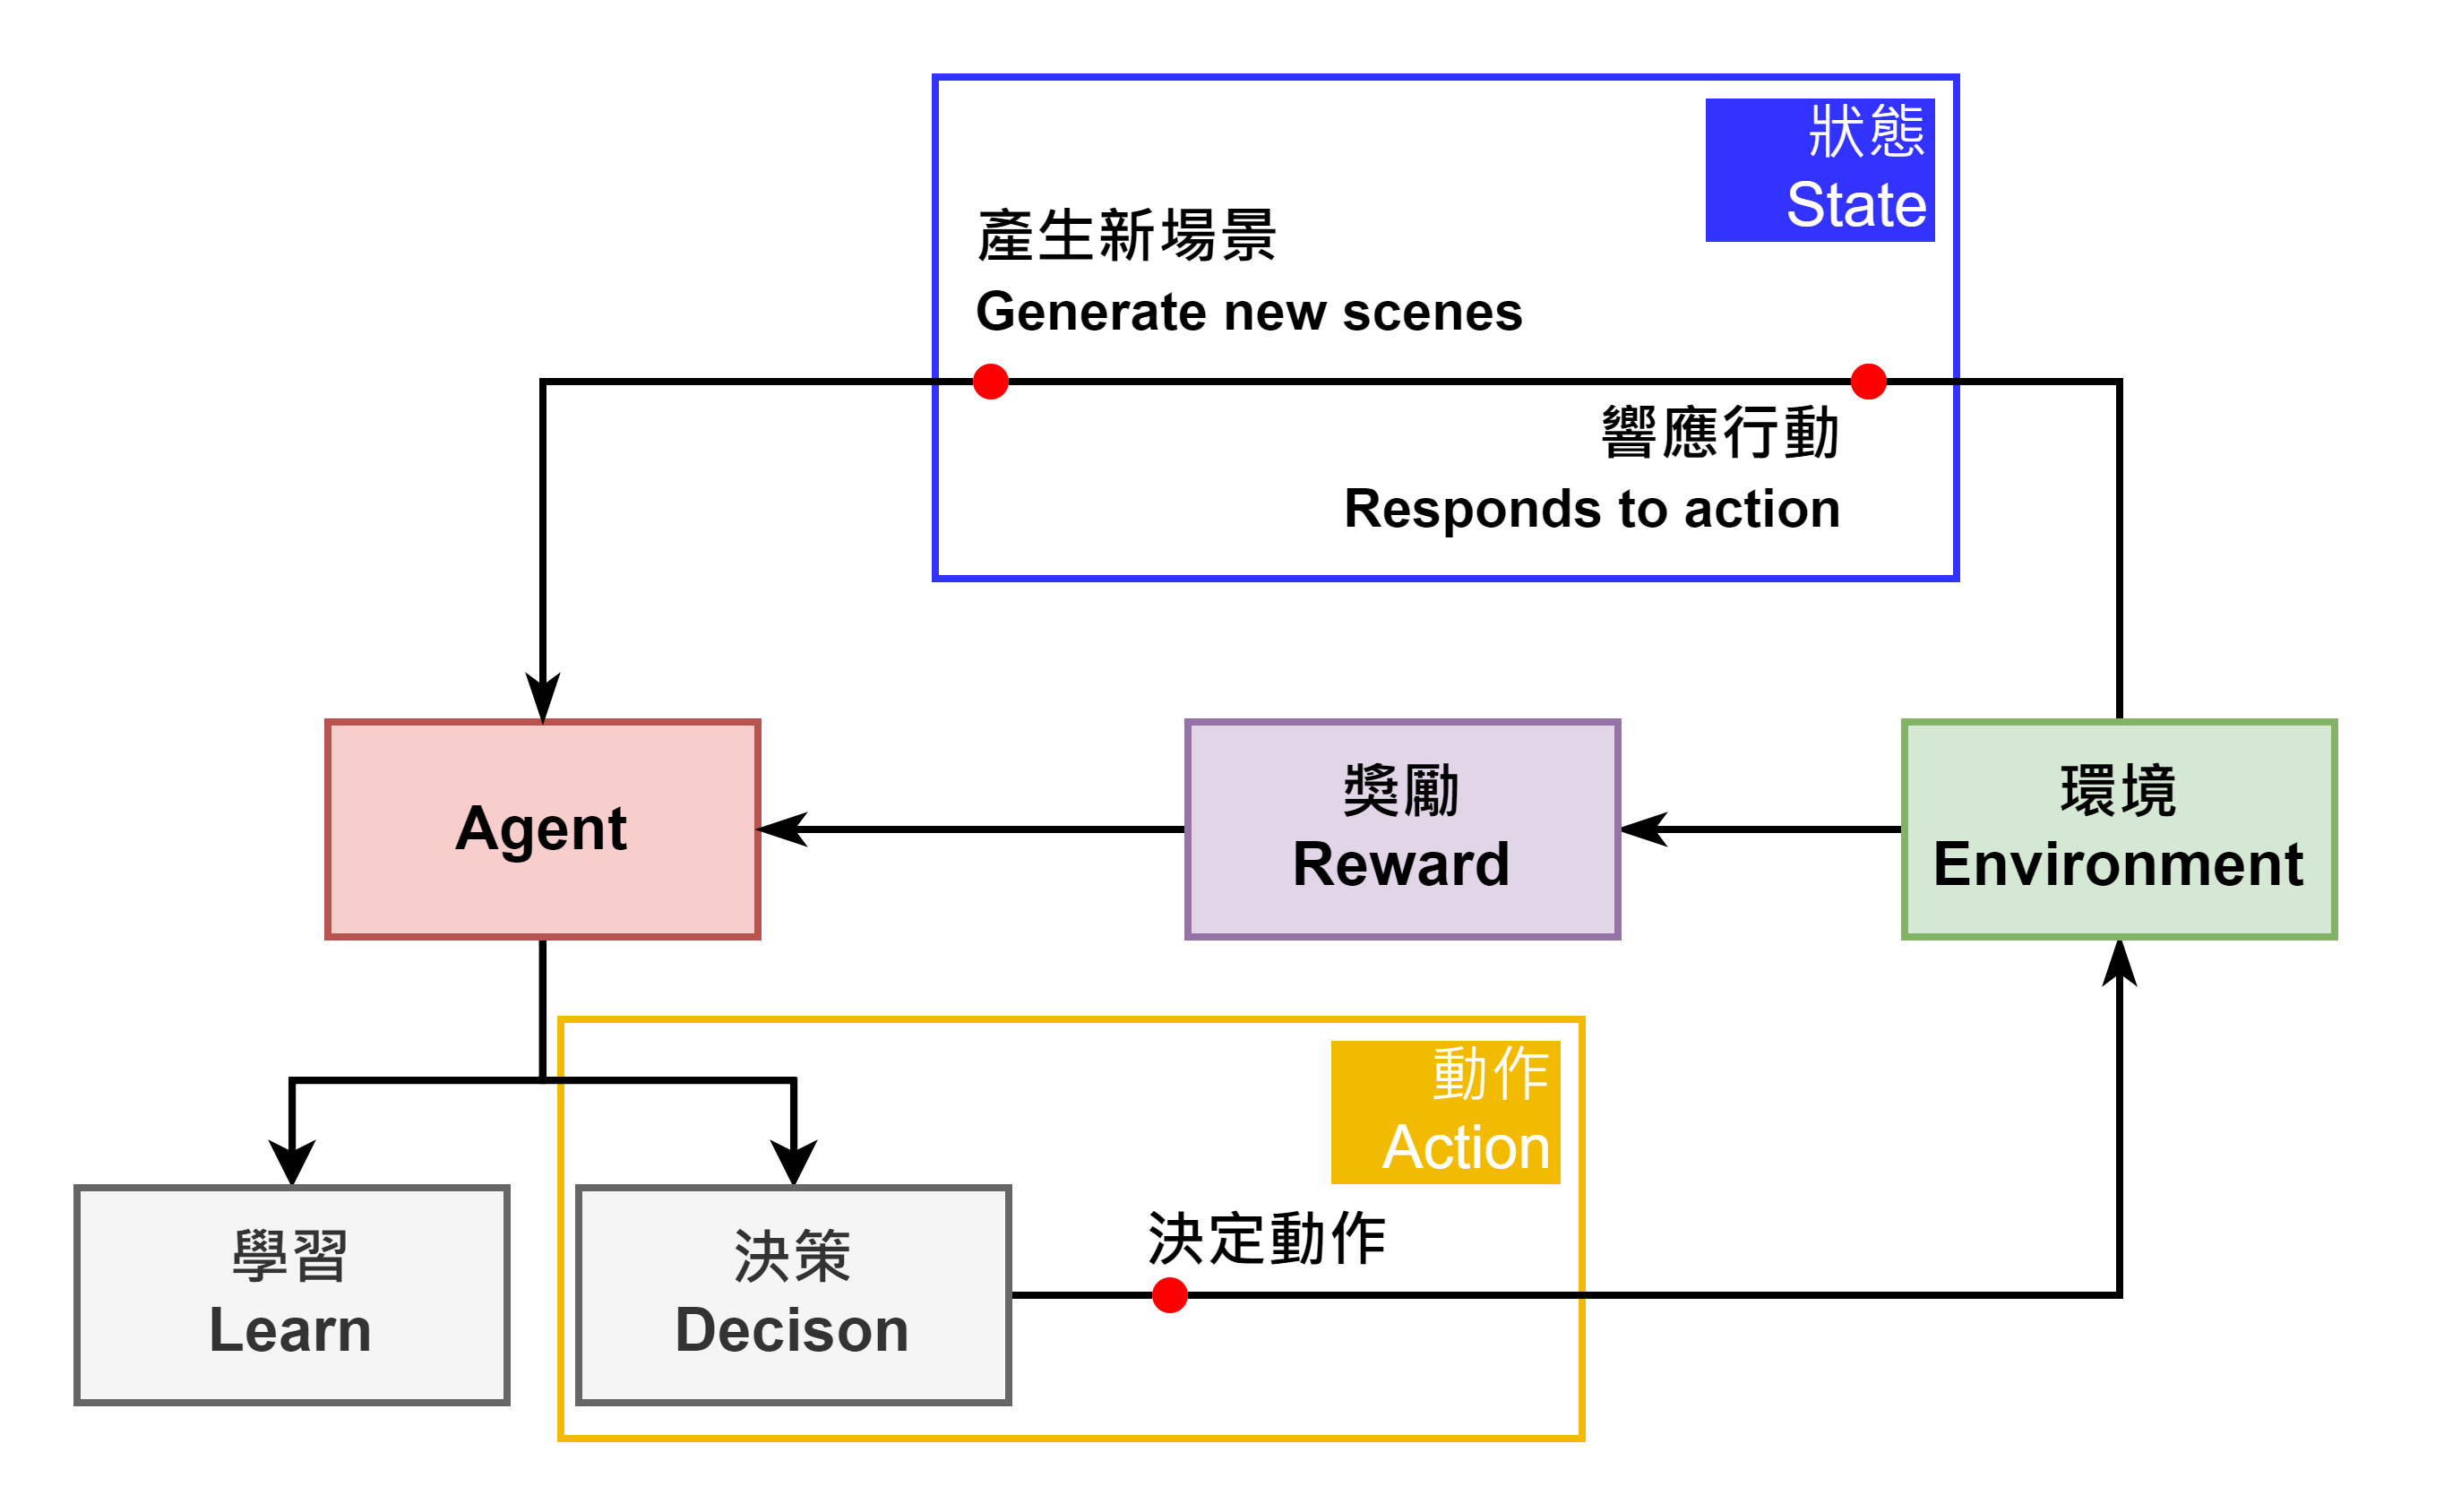
\includegraphics[width=15cm]{The_entire_interaction_process}
\caption{\Large 整個互動過程}
\label{整個互動過程}
\end{center}
\end{figure}
 如(圖.\ref{整個互動過程}) agent會透過輸入的狀態來決定採取何種行為(動作),並試圖採取獲得最高獎勵的行動。當agent開始與環境互動時,agent會透過當前狀態來決定將採取的行動,在agent採取行動後,環境的狀態也因此而改變,若agent採取行動後所到達我們所要的狀態就會得到獎勵,反之則會給予懲罰。在場景裡透過反覆的訓練,讓強化學習的行為漸漸趨近預期的目標。\\
%=----Different Terms in Reinforcement Learning----------=%
 強化學習中有兩個很重要的常數:$\gamma$和$\lambda$。\\
 
$\gamma$會影響所獲得的獎勵。$\gamma$又稱為衰減因子,正常狀態下為小於1的常數用於每個狀態改變,當狀態改變時為時常數。$\gamma$允許使用者在每個狀態給予不同形式的獎勵(這種狀況下$\gamma$為0),如果著重在長期的決策時,獎勵就不受決策順序所影響(此時$\gamma$為1)\\

$\lambda$一般在我們處理時間差異問題時使用。 這是涉及更多地連續狀態的預測。在每個狀態中$\lambda$值的增加代表演算法正在快速學習。\\
%------------------圖片可共用----------------------%
\iffalse
\begin{figure}[hbt!]
\begin{center}
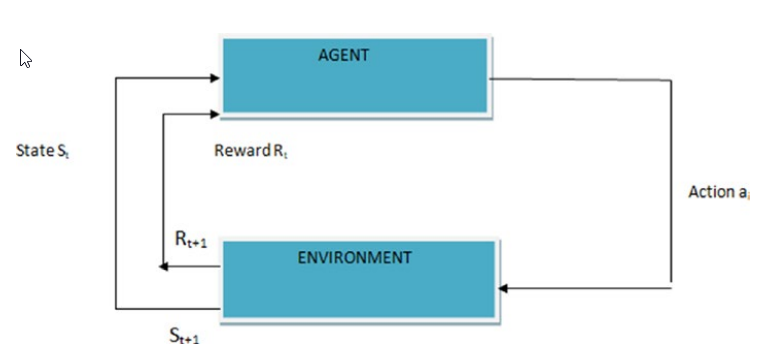
\includegraphics[scale=0.74]{ Reinforcement_Learning_interactions}
\caption{\Large Reinforcement Learning interactions}
\end{center}
\end{figure}
\fi
%=----Interactions with Reinforcement Learning------------=%

強化學習的互動是透過agent和環境之間的互動會產生獎勵,agent採取行動,導致狀態改變是一種強化學習實現如何將情況映設為行動的方法,從而找到最大化獎勵的方法,機器或機器人不會像其他機器學習形式的機器人那樣被告知要採取哪些行動。\\

獎勵的目的與運作以獎勵的方式誘導機器採取我們所期望的動作,機器會採取最大化獎勵的方式,因此可將目的定為最大獎勵,以吸引機器執行期望做的行為。\\

\begin{figure}[hbt!]
\begin{center}
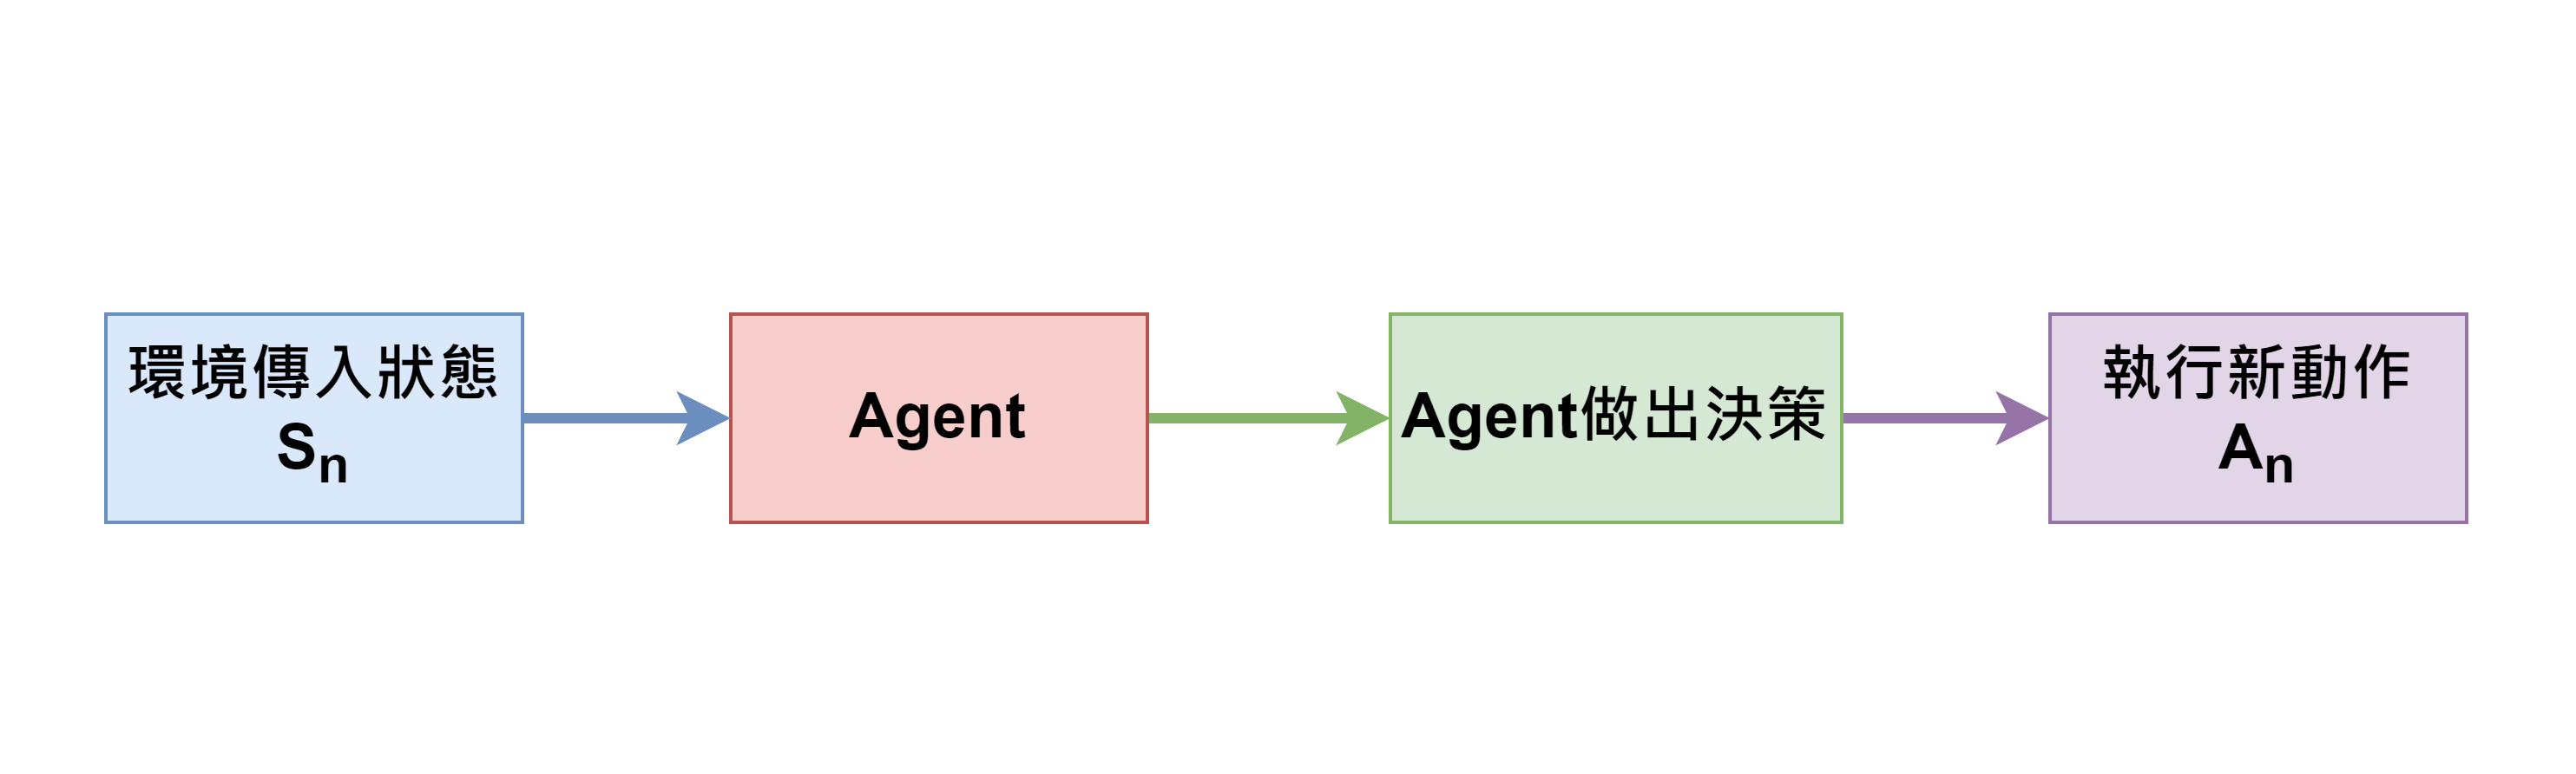
\includegraphics[width=15cm]{agent}
\caption{\Large agent}
\label{agent}
\end{center}
\end{figure}
%=----Agents------------=%
\begin{flushleft}
強化學習的環境:\\
\end{flushleft}
強化學習中的環境由某些因素組成,會對agent產生影響,agent必須根據環境適應各種因素,並做出最佳決策,這些環境可以是各種形式,其中包括2D、3D或是真實世界。強化學習的環境具有確定性、可觀察性,可以是離散或是連續的狀態,則agent可以是單一或多個所組成。\\
\subsection{馬可夫決策}
\begin{itemize}
\item Markov Chain\\
 馬可夫鏈(Markov Chain)主要是狀態變化的隨機過程(stochastic process)和馬可夫屬性(Markov property)結合。隨機過程(stochastic process)狀態隨著時間變化,而狀態的變化存在著雖機性,並以數學模式表示。馬可夫屬性(Markov property)指在目前以及所有過去事件的條件下,任何未來事件發生的機率,和過去的事件不相關僅和目前狀態相關。當前決策只會影響下個狀態,當前狀態轉移(action)到其他狀態的機率會有所差異。\\
\item Markov Reward Process\\
\begin{itemize}
\item action 到指定狀態會獲得獎勵。
$$R(s_t=s) = \mathbb{E}[r_t|s_t = s]$$
$$\gamma \in [0, 1]$$
\item Horizon:
在無限的狀態以有限的狀態表示。
\item Return:
越早做出正確決策獎勵越高。
$$G_t = R_{t+1}+\gamma R_{t+2}+\gamma^2 R_{t+3}+\gamma^3 R_{t+4}+...+\gamma^{T-t-1} R_{T}$$
\item State value function(決策價值):
$$V_t(S) = \mathbb{E}[G_t|s_t = s]$$
$$P(s_{s+1}=s'|s_t=s,a_t=a)$$
\end{itemize}
\item Discount Factor ($\gamma$)
獎勵衰減有幾種作法:第一種,越早做出有獎勵的決策,獎勵越高:第二種,做出有價值的決策$\gamma = 1$,不分決策順序先後;第三種,無用的決策$\gamma = 0$,不會得到獎勵。\\
以Bellman equation的方式描述互動關係狀態:\\
$$V(s) = R(s)+\gamma\sum_{s'\in S}P(s'|s)V(s')$$
\begin{center}
$R(s)$:立即獎勵\\
$\gamma\sum_{s'\in S}P(s'|s)V(s')$:未來獎勵衰減總和
\end{center}
Anaytic solution(分析性解法),MRP的分析性解法:
$$V = (1-\gamma P)^{-1}R$$
Bellman equation及Anaytic solution的方式只適合小的MRP(個數比較少的),矩陣複雜度為$O(N^3)$,N為狀態個數。若要計算大型的MRP會使用疊代法:動態規劃(Dynamic programming)、Temporal-Difference learning和Mote-Carlo evaluation以評估採樣的方式:
$$g = \sum_{i=t}^{H-1}\gamma^{1-t}r_i$$
$$G_t \leftarrow G_t+g,  i \leftarrow i+1$$
$$V_t(s) \leftarrow \frac{G_t}{N}$$
\item Markov Decision Process在MRP中加入決策(decision)和動作(action)
\begin{itemize}
\item S:state 狀態
\item A:action 動作
\item P:狀態轉換
$P(s_{s+1}=s'|s_t=s,a_t=a)$
\item R:獎勵,取決於當前狀態和動作會得到相對應的講勵
$$R(s_t=s, a_t=a) = \mathbb{E}[r_t|s_t, a_t=a]$$
\item D:折扣因子(discount factor)
$$\gamma \in [0,1]$$
\end{itemize}
\end{itemize}

\begin{flushleft}
policy(決策):可以是一個決策行為的機率或確定執行的行為,若以數學方程式表示:
$$\pi (a|s) = P(a_t=a|s_t=s)$$
\newpage

MRP和MDP方程式互相轉換:\\
\end{flushleft}
%=========表格=========%
\begin{center}
\begin{tabular}[c]{ccc}    
%\multicolumn{1}{r}{MRP}
 MRP & $\longleftrightarrow$ & MDP\\
\hline
$P^{\pi}(s's)$ & = & $\sum_{a\in A}\pi (a|s)P(s'|s, a)$\\
$P^{\pi}(s)$ & = & $\sum_{a\in A}\pi (a|s)P(s, a)$\\
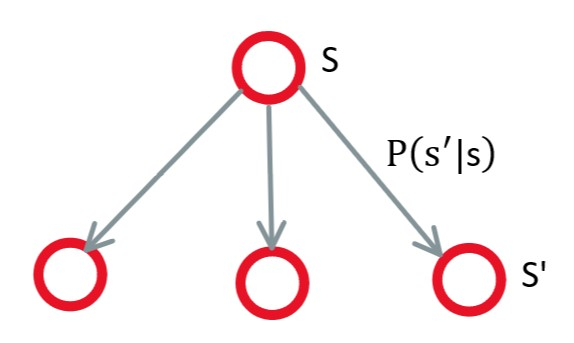
\includegraphics[height=3cm]{MRP}&&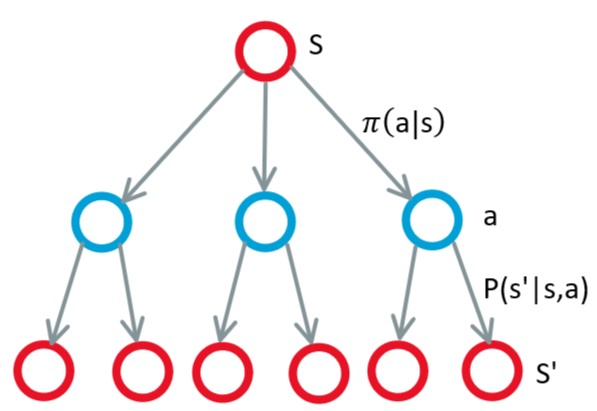
\includegraphics[height=3cm]{MDP}\\
\hline
\end{tabular}
\end{center}
\hspace{15pt}
 
state value function(狀態值方程式)$v^{\pi}(s)$\\
$$v^{\pi}(s) = \mathbb{E}[G_t|s_t=s]$$
$$= \mathbb{E}[R_{t+1}+\gamma v^{\pi}(s_{t+1})|s_t=s]$$
$$= \sum_{a\in A}\pi (a|s)q^{\pi}(s, a)$$
\begin{figure}[hbt!]
\begin{center}
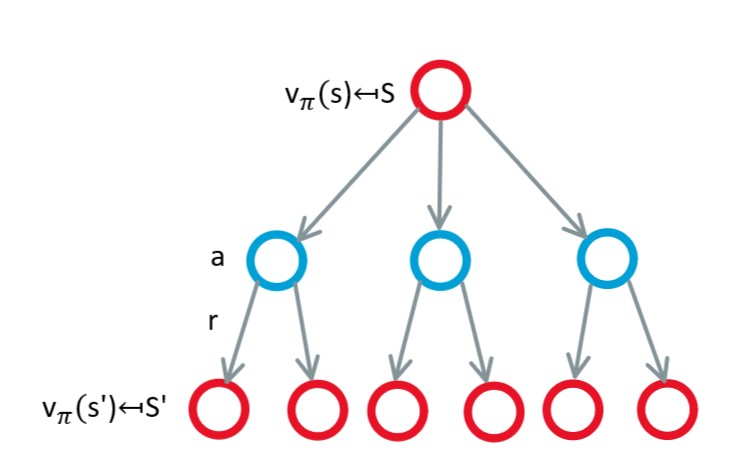
\includegraphics[width=8cm]{s_to _s}
\caption{$v^{\pi}$程序圖}
\label{fig.s_to_s}
\end{center}
\end{figure}
$$v^{\pi}(s) = \sum_{a\in A}\pi (a|s)(R(s, a)+\gamma \sum_{s'\in s}P(s'|s, a)v^{\pi}(s'))$$
\newpage
state value function(狀態值方程式)$q^{\pi}(s)$
$$v^{\pi}(s) = \mathbb{E}[G_t|s_t=s]$$
$$= \mathbb{E}[R_{t+1}+\gamma v^{\pi}(s_{t+1})|s_t=s]$$
$$= \sum_{a\in A}\pi (a|s)q^{\pi}(s, a)$$
\begin{figure}[hbt!]
\begin{center}
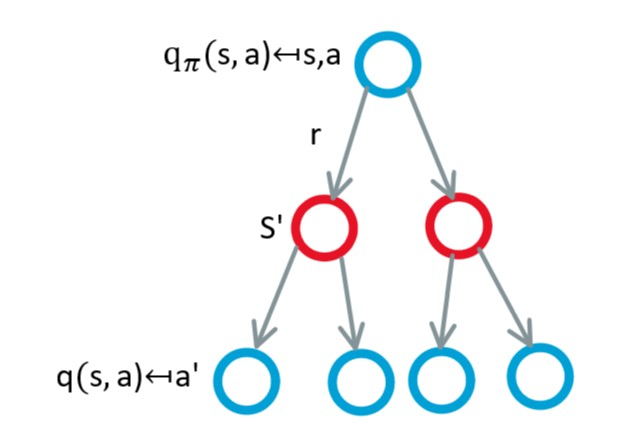
\includegraphics[width=8cm]{Q_pi function}
\caption{$q^{\pi}$程序圖}
\label{fig.q_pi}
\end{center}
\end{figure}
$$q^\pi(s, a)=R(s, a)+\gamma\sum_{s'\in S}P(s'|s, a)\sum_{a'\in A}\pi(a'|s')q^{\pi}(s', a')$$
\newpage
\section{Policy Gradient理論}
\begin{figure}[hbt!]
\begin{center}
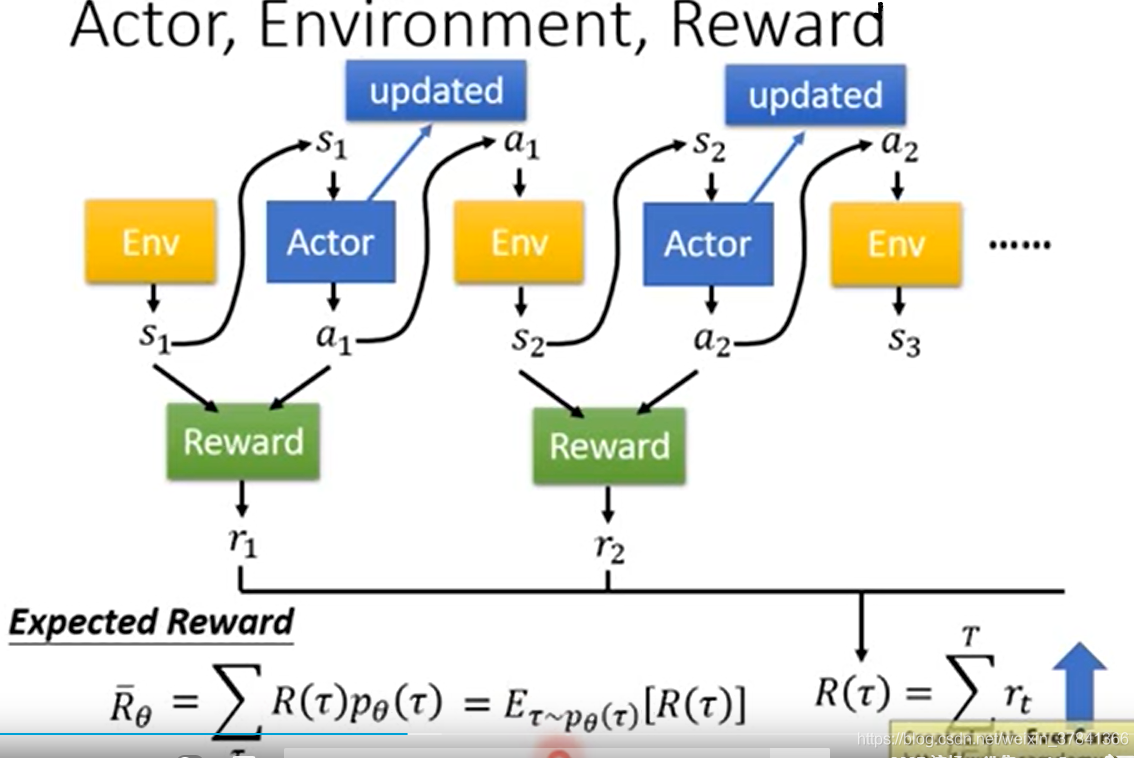
\includegraphics[width=15cm]{policy gradient原理}
\caption{\Large Policy Gradient原理}
\label{Policy Gradient原理}
\end{center}
\end{figure}

Policy Gradient主要目的是直接對決策進行建模與優化。該決策(policy)通常使用參數化函數建模,獎勵(目標)函數的值取決於此決策,可以應用各種算法來優化,以獲得最佳獎勵。(參數化:當軟體建置於一給定環境時,再依該環境的實際需求填選參數,即可成為適合該環境。)\\
參數介紹[\ref{R.Policy Gradient}]:\\
$\pi$:policy\\
s:狀態(States)。\\
a:動作(Actions)。\\
r:獎勵(Rewards)。\\
$S_t,A_t,R_t$:一個軌跡時間步長't'的State,Action and Reward。 \\
$\gamma$:衰減因子(Discount Factor);懲罰未來的不確定獎勵(reward)。\\
$G_t$:回傳衰減後的未來獎勵(Discounted future reward)$G_t = \sum_{k=0}^{\infty} \gamma^k R_{t+k+1}$\\
$P(s', r \vert s, a)$:伴隨著現在狀態(state)的a和r,前往下一個狀態s'的轉移機率矩陣(單階)。\\
$\pi(a \vert s)$:隨機策略(agent的行為策略)。\\
$\mu(s)$:確定的策略;我們還使用不同的字母將其標記為$ \pi(s)$,以提供更好的區分,以便我們可以輕鬆判斷策略是隨機的還是具有確定性的\\
$V(s)$:'狀態值函數'測量狀態的預期收益(報酬率)\\
$V^\pi(s)$:根據policy的狀態值函數$V^\pi (s) = \mathbb{E}_{a\sim \pi} [G_t \vert S_t = s]$\\
$Q(s, a)$:行為值函數,評估一對狀態和動作的預期收益。\\
$Q^\pi(s, a)$:根據policy的行為值函數$Q^\pi(s, a) = \mathbb{E}_{a\sim \pi} [G_t \vert S_t = s, A_t = a]$。\\
$A(s, a)$:Advantage Function,$A(s, a) = Q(s, a) - V(s)$:像是另一種版本的Q-value,由狀態值為基準降低方差。\\
reward function的值:取決於策略,可應用各種算法優化$\theta$,獲得最佳獎勵。\\[5pt]
$$J(\theta) 
= \sum_{s \in \mathcal{S}} d^\pi(s) V^\pi(s) 
= \sum_{s \in \mathcal{S}} d^\pi(s) \sum_{a \in \mathcal{A}} \pi_\theta(a \vert s) Q^\pi(s, a)$$\\

Policy Gradient 通過反覆評估梯度來最大化預期的總獎勵(reward)\\[5pt]
$g = \nabla_\theta\mathbb{E}[\sum_{t=0}^\infty r_t]$ ; $g = \mathbb{E}[\sum_{t=0}^\infty\psi_t\nabla_\theta log\pi_\theta(a_t \vert s_t)]$\\[5pt]
\begin{Large}{$\psi_t$ 可能方法為下列:}\end{Large}
\begin{itemize}
\item $\sum_{t=0}^\infty r$:決策軌跡的獎勵總和。
\item $\sum_{t^{'}=t}^\infty r^{'}$: 根據動作(action)的獎勵(reward) $a_t$。\\
標準表示式:$\sum_{t^{'}=t}^\infty r_t^{'}-b(s_t)$
\item $Q^\pi(s_t,a_t)$:state-action value function。
\item $A^\pi(s_t,a_t)$:Advantage Function。
\item $r_t+V^\pi(s_t+1)-V^\pi(s_t)$:TD residual。
\end{itemize}
公式使用定義[\ref{R.Policy Gradient}]:\\[5pt]
$V^\pi(s_t) = \mathbb{E}_{s_{t}+1:\infty,a_{t}:\infty}[\sum_{l=0}^\infty r_t+l]$\\[5pt]
$Q^\pi(s_t,a_t) = \mathbb{E}_{s_{t}+1:\infty_,a_{t}+1:\infty}[\sum_{l=0}^\infty r_t+l]$\\[5pt]
$A^\pi(s_t,a_t) = Q^\pi(s_t,a_t)-V^\pi(s_t)(Advantage Function)$\\[5pt]

\subsection{Actor Critic}
原始的policy gradient沒有偏差,但方差大;所以提出了許多以下算法來減少方差,同時保持偏差不變:\\[5pt]
$$g = \mathbb{E}[\sum_{t=0}^\infty\psi_t\nabla_\theta log\pi_\theta(a_t \vert s_t)]$$\\[5pt]
Actor-Critic:減少原始政策中的梯度方差包括兩個模型\\[5pt]
Critic:更新值函數參數w,根據算法,它可以是操作值$ Q_w$($a \vert s$)或狀態值$V_w$($s$) \\[5pt]
Actor:按照Critic的建議,將策略參數 $\theta$ 更新為 $\pi_\theta$($a \vert s$)\\[5pt]
\begin{Large}
它如何在簡單的行動價值參與者批評中發揮作用:
\end{Large}
\begin{itemize}
\item 隨機的初始化 s,$\theta$,w ;取樣 a $\sim
\pi_\theta(a \vert s)$
\end{itemize}
\begin{itemize}
\item For $t =1 \sim T:$ 
\begin{enumerate}[1]
\item 取樣 reward $r_t$ $\sim$ $R(s,a)$ 隨後下一階段 $s'$ $\sim$ $P(s'\vert s,a)$ 
\item 樣本的下一個動作 $a' \sim$ $\pi_\theta(a'\vert s')$
\item 更新 policy 參數 $\theta$ :\\
$$\theta\leftarrow\theta+\alpha_\theta Q_w(s,a)\nabla_\theta ln\pi_\theta(a\vert s)$$
\item 計算校正 (TD error)對於時間t的動作值:\\
$$\delta = r_t + \gamma Q_w(s',a')-Q_w(s,a)$$
並使用它來更新操作action - value function:\\
$$w\leftarrow w+\alpha_w \delta \nabla_w Q_w(s,a) $$
\item 更新 $a\leftarrow a'$ 和 $ s \leftarrow s'$ ; 學習率:$a_\theta$ 和 $a_w$。
\end{enumerate}   
\end{itemize}\newpage

\iffalse
\subsection{Policy Gradient Theorem}
Policy Gradient 通過反覆估計梯度來最大化預期的總reward\\[5pt]
$g = \nabla_\theta\mathbb{E}[\sum_{t=0}^\infty r_t]$ ; $g = \mathbb{E}[\sum_{t=0}^\infty\psi_t\nabla_\theta log\pi_\theta(a_t \vert s_t)]$\\[5pt]
\begin{Large}{$\psi_t$ 可能方法為下列:}\end{Large}
\begin{itemize}
\item $\sum_{t=0}^\infty r$:決策軌跡的獎勵總和。
\item $\sum_{t^{'}=t}^\infty r^{'}$: 根據動作(action)的獎勵(reward) $a_t$。\\
標準表示式:$\sum_{t^{'}=t}^\infty r_t^{'}-b(s_t)$
\item $Q^\pi(s_t,a_t)$:state-action value function。
\item $A^\pi(s_t,a_t)$:Advantage Function。
\item $r_t+V^\pi(s_t+1)-V^\pi(s_t)$:TD residual。
\end{itemize}
公式使用定義:\\[5pt]
$V^\pi(s_t) = \mathbb{E}_{s_{t}+1:\infty,a_{t}:\infty}[\sum_{l=0}^\infty r_t+l]$\\[5pt]
$Q^\pi(s_t,a_t) = \mathbb{E}_{s_{t}+1:\infty_,a_{t}+1:\infty}[\sum_{l=0}^\infty r_t+l]$\\[5pt]
$A^\pi(s_t,a_t) = Q^\pi(s_t,a_t)-V^\pi(s_t)(Advantage Function)$\\[5pt]
\section{類神經網路中強化學習的應用}
\begin{figure}[hbt!]
\begin{center}
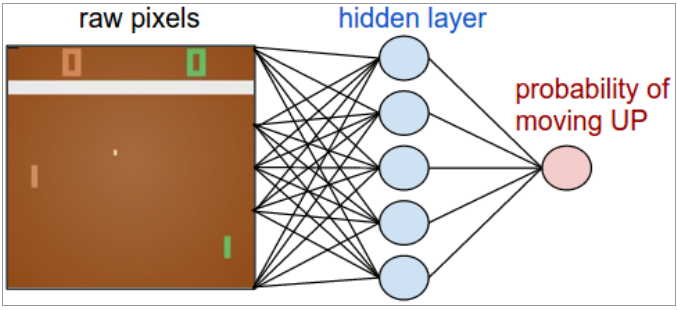
\includegraphics[scale=0.74]{network}
\caption{實際兩層神經網路}
\end{center}
\end{figure}

 我們將定義一個可以執行玩家(agent)的類神經網路,該網路將獲取遊戲狀態並決定我們應該做什麼(向上移動或向下移動我們使用一個2層神經網路,該網路獲取原始圖像像素(100,800個數字(210*160*3)),並生成一個表示上升概率的數字。 使用隨機策略是標準做法,這意味著我們只會產生向上移動的可能性,每次迭代時,我們都會從該分布中採樣(即扔一枚有偏見的硬幣)已獲得實際移動。\\

\subsection{監督式學習}
\begin{figure}[hbt!]
\begin{center}
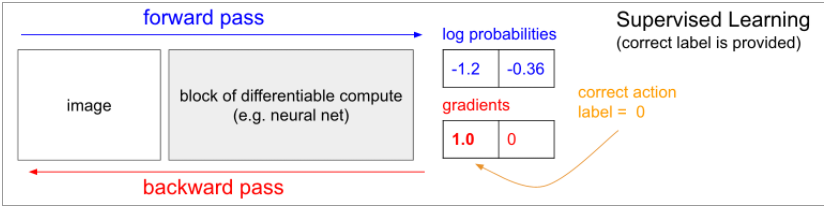
\includegraphics[scale=0.74]{supervising_learning}
\caption{監督式學習}
\end{center}
\end{figure}

 在我們深入探討 Score Function 解決方案之前,需要簡短介紹有關監督學習的知識,因為正如看到的,與我們架構類似,在普通的監督學習中,我們會將圖像傳送到網路,並獲得一概率值,例如對於兩個類別的上和下。 這裡顯示的是向上和向下對數概率(-1.2,-0.36),而不是原始機率(在這個情況下,是30$\%$和70$\%$),因為我們總是優化正確標籤的對數概率(這使我們的演算法更好,並等效於優化原始概率,因為對數是單調的),而在監督學習中,我們將可以獲取標籤,例如:
我們可能被告知現在正確的做法是向上運動(標籤0),在執行過程中,我們將以上的對數機率輸入1.0的梯度,然後運行反向傳播來計算梯度向量$Wlogp(y=UP|x)$這個梯度將告訴我們應如何更改百萬個參數中的每個參數,使網路預測往上的可能性更高,例如:網路中的百萬個參數之一可能具有-2.1的梯度,這意味著如果我們將該參數增加一個小的正值(例如0.001),則往上的對數機率將因2.1*0.001而降低(由於負號而減少),如果我們隨後更新了參數,當之後遇到非常相似的圖像時(也就是環境狀況),我們的網路現在更有可能預測往上。\\

\subsection{對數導數技巧}
 機器學習涉及操縱機率。這個機率通常包含歸一化概率或對數概率。能加強解決現代機器學習問題的關鍵點,是能夠巧妙的在這兩種型式間交替使用,而對數導數技巧就能夠幫助我們做到這點,也就是運用對數導數的性質。\\
 
\subsection{為什麼選擇score function 算法}
 多篇論文已經廣泛使用了ATARI遊戲並結合了DQN(它是一種在強化學習算法裡,知名度較高的),事實證明,Q-Learning並不是一個很好的算法,實際上大多數人比較喜歡使用Policy Gradients,包括原始DQN論文的作者,他們在調優後顯示Policy Gradients比Q-Learning運作得更好,首選PG是因為它是端到端的:有一個明確的政策和一種有原則的方法可以直接優化預期的回報。但是礙於時間考量,而選擇了類似PG的算法,也就是score function gradient estimator(取用Andrej Karpathy),從像素開始,通過類神經網路加上強化學習結合ATARI遊戲(Pong),在整個過程使用numpy運算,作為訓練工具。\\ 
 
\subsection{Score Functions}
 對數導數技巧的應用規則是基於參數$\theta$梯度的對數函數$p(x:\theta)$,如下:\\
$$\nabla_\theta logp(x:\theta)=\frac{\nabla_\theta p(x:\theta)}{p(x:\theta)}$$\\
$p(x:\theta)$是likelihood ; function參數$\theta$的函數,它提供隨機變量x的概率。在此特例中,$\nabla_\theta logp(x:\theta)$被稱為Score Function,而上述方程式右邊為score ratio(得分比)。\\
score function具有許多有用的屬性:\\

\begin{itemize}
\item 最大概似估計的中央計算。最大概似是機器學習中使用的學習原理之一,用於廣義線性回歸、深度學習、kernel machines、降維和張量分解等,而score出現在這些所有問題中。
\end{itemize}
\begin{itemize}
\item  score的期望值為零。對數導數技巧的第一個用途就是證明這一點。\\
$$\mathbb{E}_{p(x; \theta)}[\nabla_\theta \log p(\mathbf{x}; \theta)] =\mathbb{E}_{p(x; \theta)}\left[\frac{\nabla_\theta p(\mathbf {x}; \theta)}{p(\mathbf{x}; \theta)} \right]$$
$$= \int p(\mathbf {x}; \theta) \frac{\nabla_\theta p(\mathbf {x}; \theta)}{p(\mathbf{x}; \theta)} dx= \nabla_\theta \int p(\mathbf{x}; \theta) dx=\nabla_\theta 1 = 0$$\\
\qquad 在第一行中,我們應用了對數導數技巧,在第二行中,我們交換了差異化和積分的順序,這種特性是我們尋求概率靈活性的類型:  它允許我們從期望值為零的分數中減去任何一項,且此修改不會影響預期得分(控制變量)。
\end{itemize}
\begin{itemize}
\item 得分的方差是Fisher信息,用於確定Cramer-Rao下限。\\
$$\mathbb{V}[\nabla_\theta \log p(\mathbf{x}; \theta)] = \mathcal{I}(\theta) =\mathbb{E}_{p(x; \theta)}[\nabla_\theta \log p(\mathbf{x}; \theta)\nabla_\theta \log p(\mathbf{x}; \theta)^\top]$$\\
我們現在可以從對數概率的梯度躍升為概率的梯度,然後返回,但是真正要解決的其實是計算困難的期望梯度,所以我們可以利用新發現的功能:score function為此問題開發另一個聰明的估計器。
\end{itemize}
\subsection{Score Function Estimators}
我們的問題是計算函數f的期望值的梯度:\\
$$\nabla_\theta \mathbb{E}_{p(z;\theta)}[f(z)] =\nabla_\theta \int p(z; \theta)f(z) dz$$
 這是機器學習中的一項常態性任務,在變數推理中進行後驗計算,在強化學習中進行價值函數和策略學習,在計算金融中進行衍生產品定價以及在運籌學中進行庫存控制等。該梯度很難計算,因為積分通常是未知的,我們計算梯度所依據的參數θ的分佈為p(z;θ),此外,當函數f不可微時,我們可能想計算該梯度,使用對數導數技巧和得分函數的屬性,我們可以更方便地計算此梯度:\\
$$\nabla_\theta \mathbb{E}_{p(z;\theta)}[f(z)] = \mathbb{E}_{p(z;\theta)}[f(z)\nabla_\theta \log p(z;\theta)]$$
\begin{figure}[hbt!]
\begin{center}
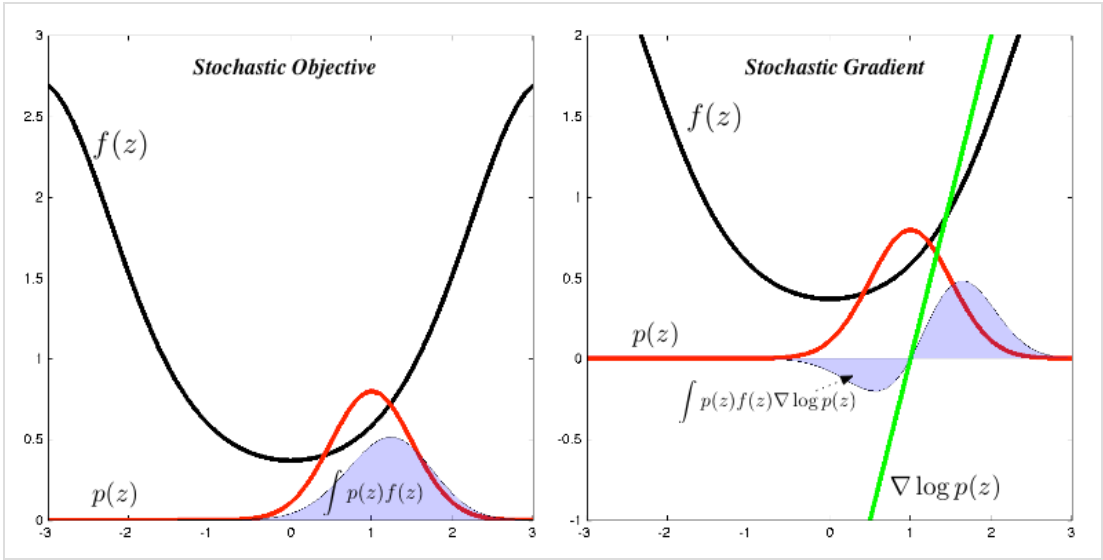
\includegraphics[scale=0.5]{gradient_change}
\caption{梯度變化}
\end{center}
\end{figure}
 讓我們導出該表達式,並探討它對我們的優化問題的影響。\\
 為此,我們將使用另一種普遍存在的技巧,一種概率恆等的技巧,在該技巧中,我們將表達式乘以1,該表達式由概率密度除以自身而形成。將特性技巧與對數導數技巧相結合,我們獲得了梯度的得分函數估計量:\\
$$\nabla_\theta \mathbb{E}_{p(z;\theta)}[f(z)]=\int\nabla_\theta p(z;\theta)f(z) dz$$
$$= \int \frac{p(z;\theta)}{p(z;\theta)}\nabla_\theta p(z;\theta)f(z) dz$$
$$=\int p(z;\theta)\nabla_\theta \log p(z;\theta)f(z) dz = \mathbb{E}_{p(z;\theta)}[f(z)\nabla_\theta \log p(z;\theta)]$$
$$=\int p(z;\theta)\nabla_\theta \log p(z;\theta)f(z) dz = \mathbb{E}_{p(z;\theta)}[f(z)\nabla_\theta \log p(z;\theta)]$$
$$\approx \frac{1}{S} \sum_{s=1}^{S}f(z^{(s)})\nabla_\theta \log p(z^{(s)};\theta) \quad z^{(s)}\sim p(z)$$\\
在這四行中發生了很多事情。在第一行中,我們交換了導數和積分。在第二行中,我們應用了概率身份技巧,這使我們能夠形成得分比, 然後使用對數導數技巧,用第三行中對數概率的梯度替換該比率。這在第四行給出了我們所需的隨機估計量,這是由蒙特卡洛計算的,方法是首先從p(z)提取樣本,然後計算加權梯度項。\\

更簡單的描述,我們有一些分佈 $p(x;\theta)$(我們使用了速記$ p \left( x \right)$ 來減少混亂),我們可以從中採樣(例如,這可能是高斯)。對於每個樣本,我們還可以評估score function f(x),該函數將樣本作為樣本並給出標量值。該方程式告訴我們,如果我們希望其樣本達到較高的分數(由f判斷),應該如何改變分佈(通過其參數θ),特別是,它看起來像:畫出一些樣本x,評估其分數f(x),並且對於每個x也評估第二項 $\nabla_\theta logp(x;θ)$,第二項是一個漸變向量為我們提供了參數空間中的方向,使分配給x的概率增加。換句話說,如果我們要在的方向上微移θ,$\nabla_\theta logp(x;θ)$,分配給x的新概率略有增加,朝這個方向移動,並將標量值加到上面$f(x)$。根據p(x)上的幾個樣本進行更新,則概率密度將朝著較高分數的方向移動,從而使得分較高的樣本更有可能出現。\\
\begin{figure}[hbt!]
\begin{center}
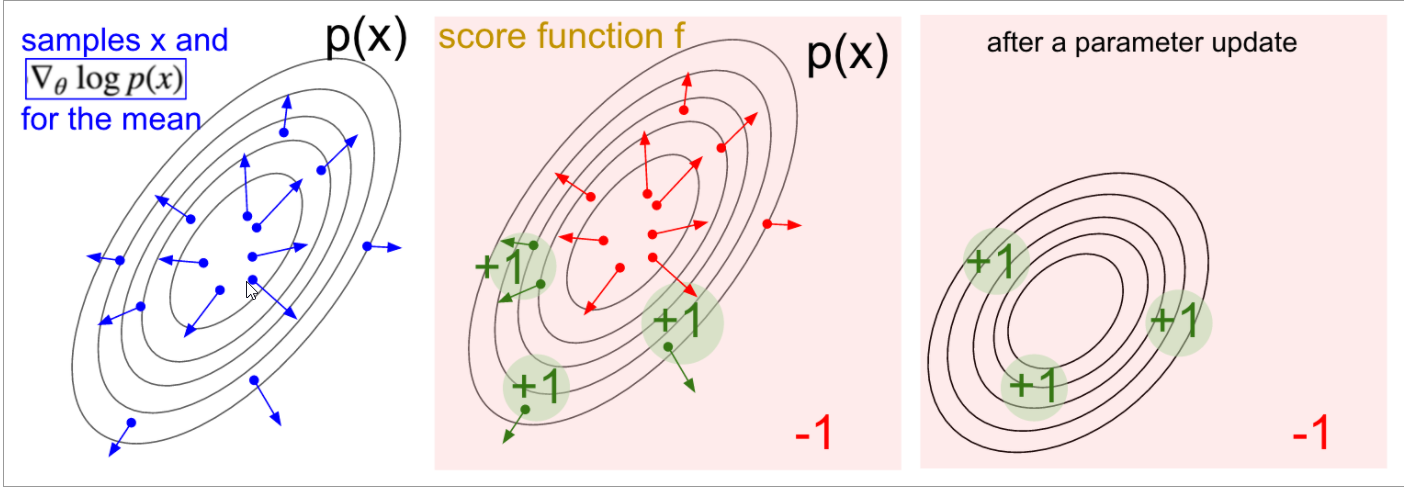
\includegraphics[scale=0.4]{figure}
\caption{Score Function可視圖}
\end{center}
\end{figure}

 Score function gradient estimator的可視化,左:高斯分佈及其中的一些樣本(藍點),在每個藍點上,我們還繪製了相對於高斯平均參數的對數概率的梯度,箭頭指示應微調分佈平均值以增加該樣本概率的方向。中間:某些得分函數的疊加,在某些小區域中除了+1之外,其他所有地方都給出-1,箭頭採用顏色區別,更新運用乘法運算,我們將平均所有綠色箭頭和紅色箭頭。右:更新參數後,綠色箭頭和反向紅色箭頭將向左移至底部。現在,根據需要,該分佈中的樣本將具有更高的預期分數。\\
\fi
\newpage
